% savequote{ \begin}[-75mm]
% Nulla facilisi. In vel sem. Morbi id urna in diam dignissim feugiat. Proin molestie tortor eu velit. Aliquam erat volutpat. Nullam ultrices, diam tempus vulputate egestas, eros pede varius leo.
% \qauthor{Quoteauthor Lastname}
% \end{savequote}
\chapter{Machine Learning methods and analysis for VELO}

This chapter is dedicated to the research of the VELO detector, and possibility of application of machine learning methods for it's purposes. Most of the scope of the work relates to the version of VELO used in runs 1 and 2 of the LHC, but it also contains studies for the upgraded VELO. Those studies have been conducted in different timespans. So for the section \ref{chap4:run12} the data used (2010-2017) doesn't contain the data that was used (2010-2018) for the analysis in sections \ref{chap4:dimred} and \ref{chap4:wtte}. The structure of sections in this chapter is keeping the chronological order of the conducted studies.

\section{Run 1 and 2 calibration analysis}
\label{chap4:run12}
% @TODO add something about those runs

\subsection{The Data}

The data used in this section comes from a timespan 2010-08-18-017-06-21, and contains 30 calibration.
It relates to the calibration data. The most significant for the VELO set of data are the following parameters: Pedestals $P$, Low Threshold $L_t$ and High Threshold $H_t$.
As discussed
%@TODO make reference
Low Threshold and High Threshold only differ in scaling factor, so in further analysis in this section only high threshold and pedestal parameters will be used. 
The most useful tool for the analysis of this dataset is the 2D histogram, with a channel number on X axis, and a parameter value on the Y axis. The color of the histogram marks the intensity, or a number of occurance of the (X,Y) pair in the dataset. When there is no occurance of a gicen pair of values, the color is set to white. The color scale is different for each of the plots, unless mentioned otherwise. The color scale in most of the plots is ommited, and it follows the intuitive rule of warmer colors meaning more occurances.
This kind of figure has prooved to be very useful, since it can aggregate multiple dimentions of the data.

Before going further a discussion of the dimentionality of the data is necessary. The VELO sensor has 2048 channels, which constitues the channel dimmention. The sensors are or $R$ and $\phi$ type, for each of the 42 modules. Those are make two additional dimentions of the data. The final one is the calibration date, which can be different in further sections.

\begin{table}[h]
\begin{center}
\begin{tabular}{ |c|c|c| }
\hline
Dimention name & Symbol & Size\\
\hline
Channel & $Ch$ & 2048\\
Sensor type & ${R, \phi}$ & 2 ($R$ or $\phi$) \\
Module number & $\#$ & 42 \\
Calibration date & $T$ & 30\\
\hline
\end{tabular}
\caption{\label{tab:velo_dimentionality}Table of dimentionality of the calibration dataset.}
\end{center}
\end{table}

We will be using the following notation to denote the slice of dataset: $ParameterType_{Ch, S, \#, T}$. Where $ParameterType$ stand for the type of the parameter like $P$ or $H_t$ and the other symbols are explained in the Table \ref{tab:velo_dimentionality}. Single symbol without values marks the use of full range of data on that dimension. Examplary notation: $P_{Ch100-Ch500, R, \#11, T}$ is a slice of R-type sensor channels from 100 to 500 in module $\#11$ in all of the calibrations.
%@TODO maybe a little bit more about why 2D histograms are useful?

\subsection{Pedestals}

The Fig. \ref{plot:part1-r-phi-pedestals} depicts all of the pedestals value in all of the dataset. The value oscillates around 520 ADC, with visible artifacts at channels 1400-1520 in R type sensor, and near channel 1750 in both sensor types. The first artifact (rangees 1400-1520) comes solemly from the sensor \#85 
% @TODO recast senor number
, visible in the Fig. \ref{plot:par1-pedestal-sensors}. This is believed to be a malfunction of the sensor in range of channels in this particular sensor. 
The other artifact near channel 1750, is believed to be coming from a design flaw, which placed a clock line too close to those channels. 
This is not a major problem, since the purpose of pedestals is to level the differences in a basic level of the signal.

\begin{figure}
    \centering
    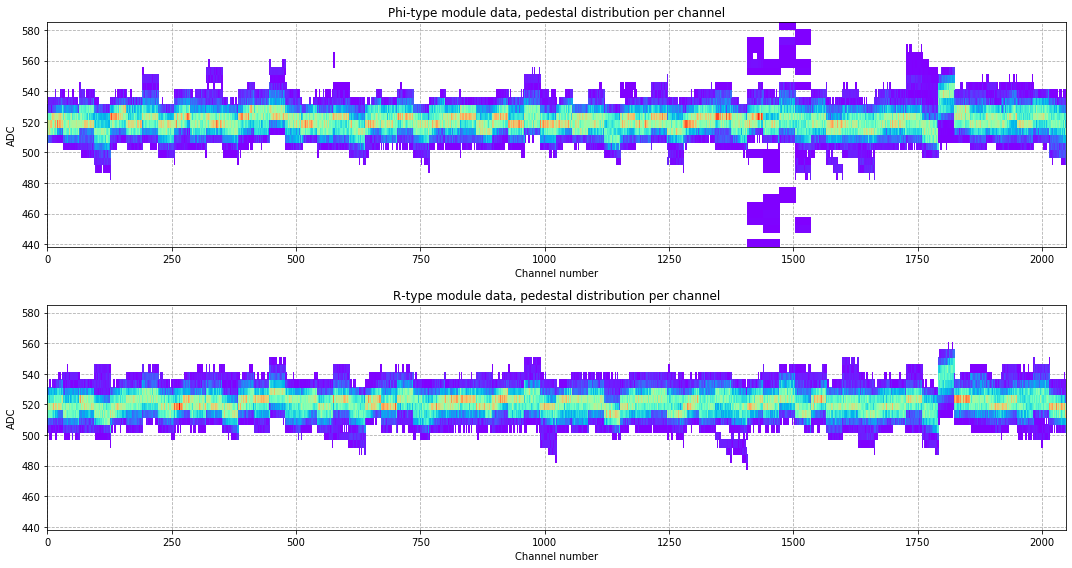
\includegraphics[width=0.5\linewidth]{figures/chapter4/calib_analysis/Part1-r-phi-pedestals.png}
    \caption{Histogram of the all of the pedestal values, across all of the calibrations The histogram above is $P_{Ch, R, \#, T}$ and the below $P_{Ch, \phi, \#, T}$).}
    \label{plot:part1-r-phi-pedestals}
\end{figure}


\begin{figure}
    \centering
    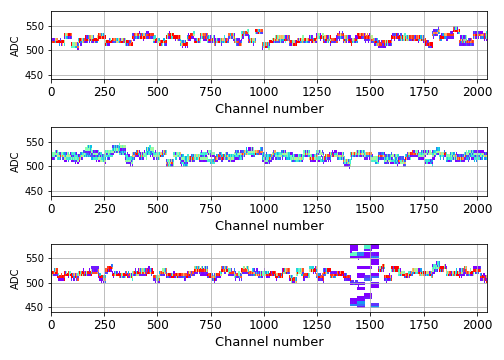
\includegraphics[width=0.5\linewidth]{figures/chapter4/calib_analysis/Part1-outliers-pedestals-cases.png}
    \caption{Pedestal plot for sensors $P_{Ch, R, \#64, T}$ $P_{Ch, R, \#35, T}$ $P_{Ch, R, \#85, T}$. $\#64$ and \#35 represent a typical pedestal values, while in \#85 there is a malfunction visible close to channel 1500.}
    %@TODO recast the sensors to their modules, and check the sensor type
    \label{plot:par1-pedestal-sensors}
\end{figure}

The radiation constantly damages the sensors, resulting in need of asjusting bias voltage
%@TODO make sure that you discuss what bias voltage is
The pedestals are actually a way of fine-tuning the levels of the signal. If the value of the pedestals would exhibit a trend this could mean that the bias voltage adjustment is not sufficient, or it doesn't give desired result. Thus, a study of the trend of the pedestals is important aspect of this analysis. The trend was calculated by fitting a line ($y=ax+b$) to the pedestal values in the time (calibration) domain. The value of the linear coefficient ($a$) which is responsible for the trend, is calculated individually for each of the channels of the detector. The distribution of this coefficient is visible in the Fig. \ref{plot:part1-pedestal-trend}. The mean value of the coefficient is $9.63e-05$ which is so close to zero that it can be assumed that there is no overall trend.
%@TODO check the dimensionality of the coefficient!!!

\begin{figure}
    \centering
    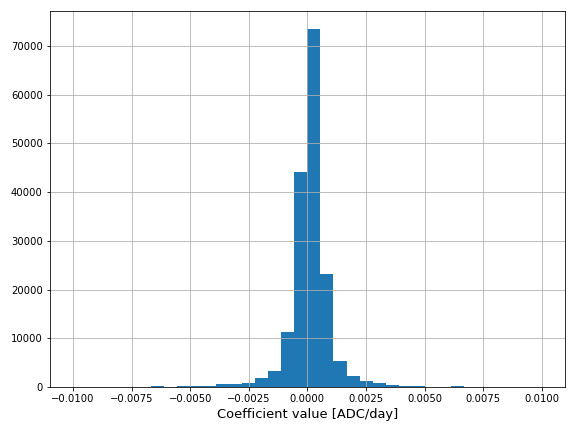
\includegraphics[width=0.7\linewidth]{figures/chapter4/calib_analysis/Part1-pedestal-trend.png}
    \caption{Histogram of linear coefficient of the pedestal trend per channel. Some of the outlyingcoefficient values have been trimmed,  and are outsidethe scope of this plot.}
    \label{plot:part1-pedestal-trend}
\end{figure}

\subsection{Threshold}

Of the two studied parameters, the high threshold parameter is the one actually responsible for the sensitivity of the detection of the hit. It is one of th many steps of filtering the signal coming from VELO. Further, the hit information is crutial for the reconstruction algorithms and particle detection and recognition. 
%@TODO maybe add a citation?
At first glance, a 2D histograms visible in Fig. \ref{plot:part2-threshold-all} is cluttered by outlying values. 
The most visible ones are near value 127 across all channels. This is actually an expected sight, as setting a value to 127 means the maximal possible value which makes the data coming from the channel unusable. This is a masking value, and occurances of those masks are discussed in detail in the next section. 
This comes from afaulty  sensor  \#67  and  dates  ’2016-11-07’  and  ’2016-11-11’,  where  the  threshold  value  reaches  400  ADC. This likely an error of that could accidentally get into the dataset, and yet there is no explanation for those values.
Moving on, we ignore those values, and limit the analysis to the range of values close to 0.

\begin{figure}
    \centering
    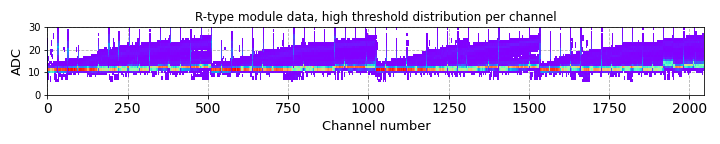
\includegraphics[width=0.7\linewidth]{figures/chapter4/calib_analysis/P2-threshold-all-zoom.png}
    \caption{High threshold distribution with header cross-talk. $H_t(Ch, \phi, \#, T)$ above and $H_t(Ch, R, \#, T)$ below.}
    \label{plot:P2-threshold-all-zoom}
\end{figure}

The Fig. \ref{plot:P2-threshold-all-zoom} depicts $H_t(Ch, R, \#, T)$ and $H_t(Ch, \phi, \#, T)$ in range of values from 0 to 30. One of the immidiatelly visible things are the vertical strips of low intensity, spaced throughout the channels. This a header cross-talk effect, in which the signal is disturbed.
% @TODO you will have to explaine the HC effect
In some cases it might be useful to exclude the channels that contain the header crosstalk effect, and the full list of the those channels is present in the appendix.
The $Ch*$ denotes all of the channels withouth the header cross-talk effect. 
% @TODO add the HC channel list and reference it here.
The reader can examine the difference of the histogram with and without header cross-talk in the Fig. \ref{plot:P2-threshold-all-zoom} and \ref{plot:P2-threshold-all-zoom-nohc}.

\begin{figure}
    \centering
    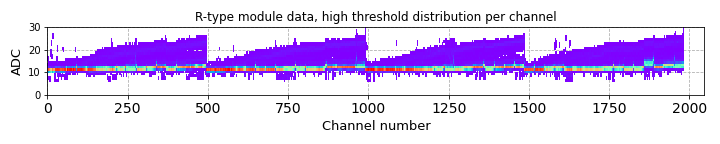
\includegraphics[width=0.7\linewidth]{figures/chapter4/calib_analysis/P2-threshold-all-zoom-nohc.png}
    \caption{High threshold distribution without header cross-talk. $H_t(Ch*, \phi, \#, T)$ above and $H_t(Ch*, R, \#, T)$ below.}
    \label{plot:P2-threshold-all-zoom-nohc}
\end{figure}


\begin{figure}
    \centering
    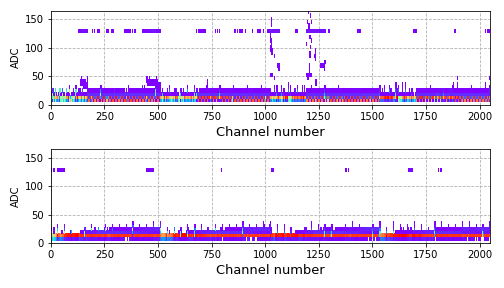
\includegraphics[width=0.7\linewidth]{figures/chapter4/calib_analysis/P2-threshold-all-r-phi.png}
    \caption{High threshold distribution of all of the calibrations, across all sensors. $H_t(Ch,\phi,\#, T)$ is above, and $H_t(Ch,\phi,\#, T)$ is the plot below.}
    \label{plot:part2-threshold-all}
\end{figure}

Another insight coming from the 2D histogram coming from the Fig. \ref{plot:P2-threshold-all-zoom-nohc} is that there are regularities of low intensity, repeating roughly every 512 channels. The periodicity of those regularities comes from the design of the sensors, and the pattern of the sitribution of that the channels and their lines.
(@TODO what lines)
More precisely they are recognised as imperfect calibrations coming from two dates  '2012-07-30', '2012-08-01'.
Those two dates are imperfect due to the power break occuring on those dates.
This imperfect calibration was influencing the sensitivity of the detector, and overall data taking.
Additionally for the purpose of outlierness analysis two calibration dates also being are recognised as imperfect 2012-08-02 and 2011-03-07.
Those occurances of the miscalibration are a direct motivation for detecting anomalies in the calibration in section \ref{chap4:outlierness}.


\begin{figure}
    \centering
    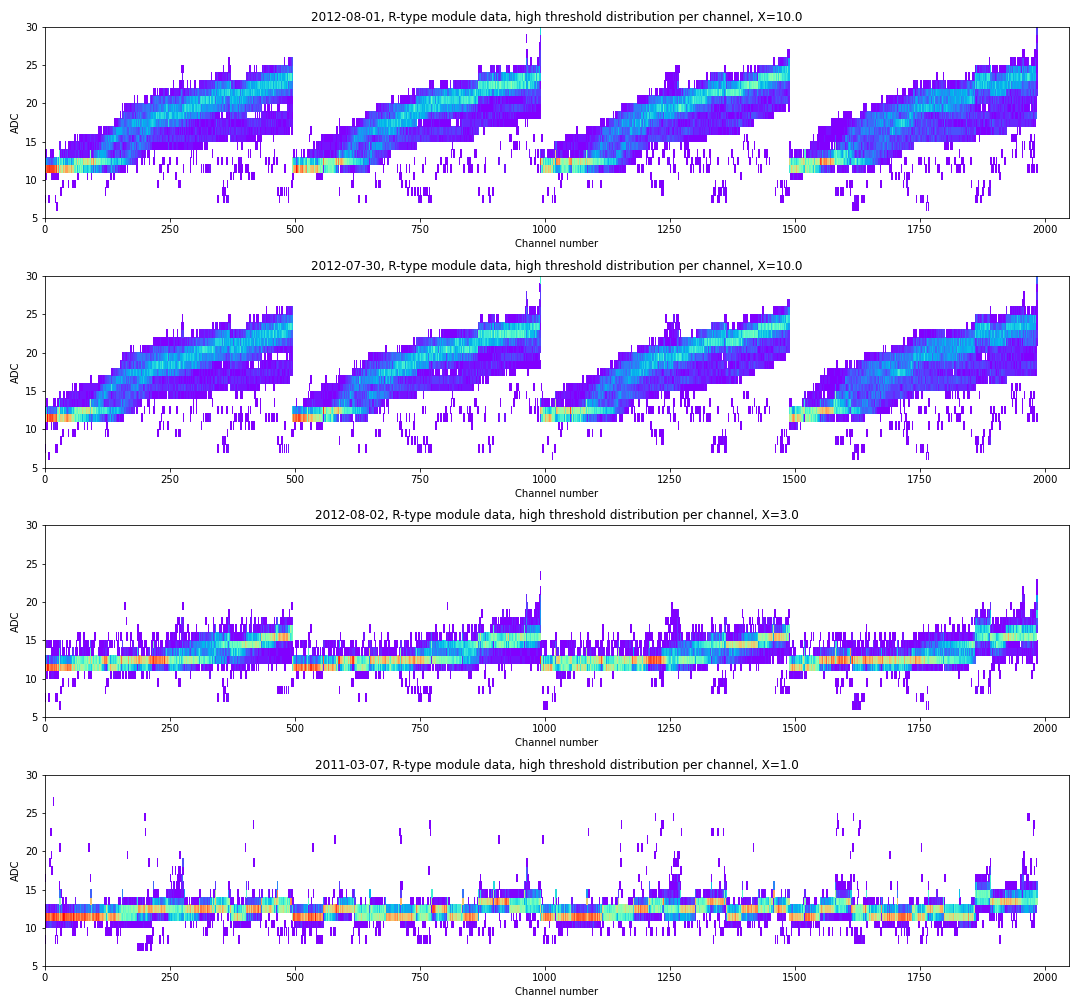
\includegraphics[width=0.6\linewidth]{figures/chapter4/calib_analysis/P2-all-bad-cals-R.png}
    \caption{Various R type calibration dates, with assigned value of outlierness.}
    \label{plot:all-bad-r}
\end{figure}

\begin{figure}
    \centering
    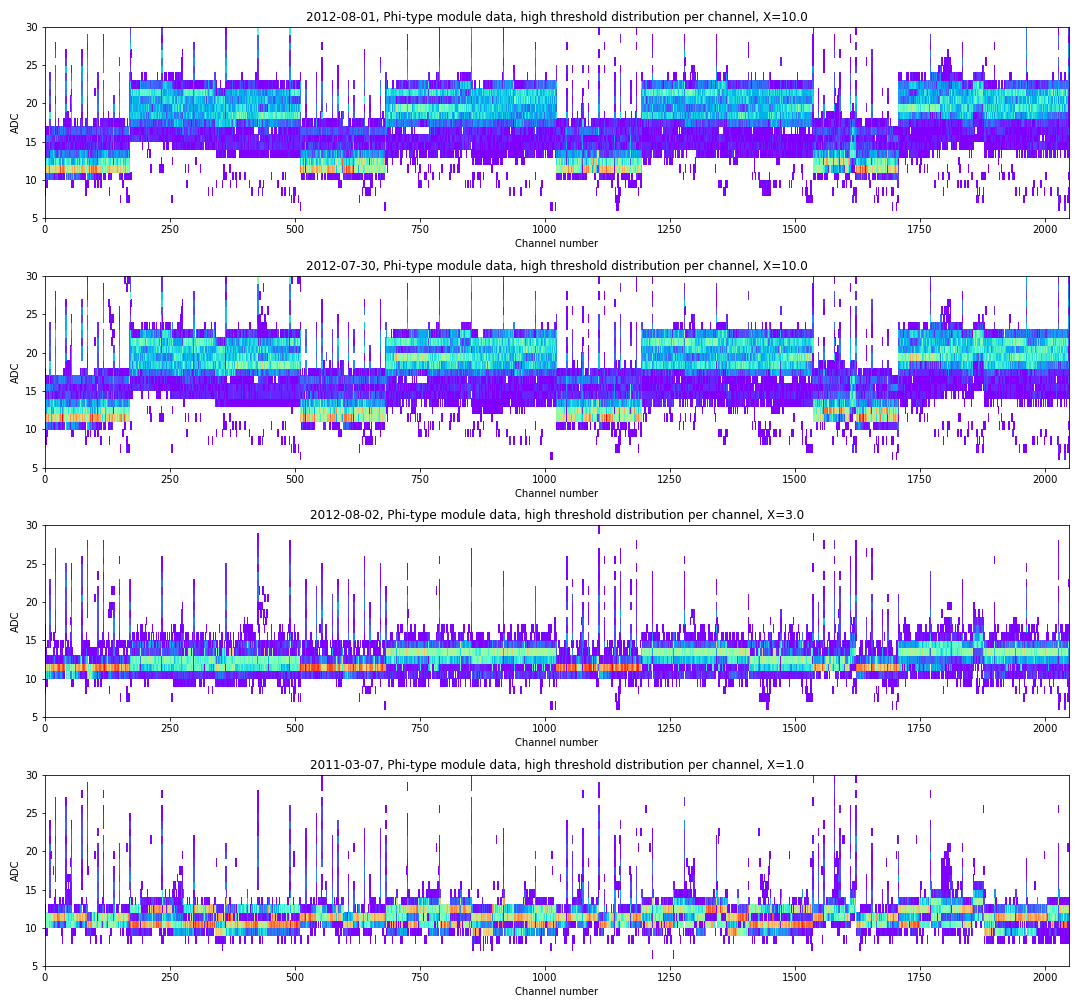
\includegraphics[width=0.6\linewidth]{figures/chapter4/calib_analysis/P2-all-bad-cals-phi.png}
     \caption{Various phi type calibration dates, with assigned value of outlierness.}
    \label{plot:all-bad-phi}
\end{figure}


\begin{figure}
    \centering
    
    \begin{subfigure}[b]{\textwidth}
    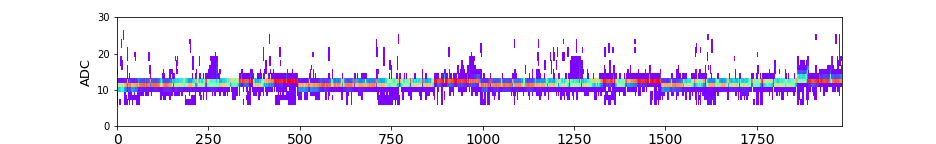
\includegraphics[width=\linewidth]{figures/chapter4/calib_analysis/P2-only-good-R.png}
    \caption{ .}
   \label{plot:only_good_r}
  \end{subfigure}
  
  \begin{subfigure}[b]{\textwidth}
    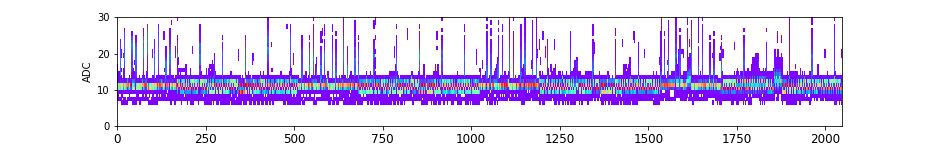
\includegraphics[width=\linewidth]{figures/chapter4/calib_analysis/P2-only-good-phi.png}
    \caption{ .}
   \label{plot:only_good_phi}
  \end{subfigure}
      \caption[All calond]{All of the calibrations, with reduced dimentionality using autoencoder and PCA.}
    \label{plot:only_good_all}
  
  \end{figure}



\subsection{Masked Values and others}



  As mentioned previously, the $H_t=127 ADC$ means that the channel is being masked.
  Setting the threshold so high, means that no hit will be registered in a given channel.
  The masks were given to the channels that exhibited exceptional noise levels.
  Their occurances are depicted in Figs \ref{plot:p3-mask-time} and \ref{plot:p3-mask-time2}.
  In  \ref{plot:p3-mask-time} the channels from all calibration are plotted as number of blocked channels per sensor in time domain.
  The important insight is that some sensors are more prone to masking channels than others, and that during the ammount of masked channels changes.
  In some cases the masked channels can go away and come back into the sensor.
  The figure \ref{plot:p3-mask-time2} depicts number of masked channels in time domain, with a sensor split.
  It is clearly visible that the total number of masked channels grows with time.
  (@TODO show that this goes in hand with total luminosity).
  This is expected as with time the negative radiation effects accumulate.

\begin{figure}
    \centering
    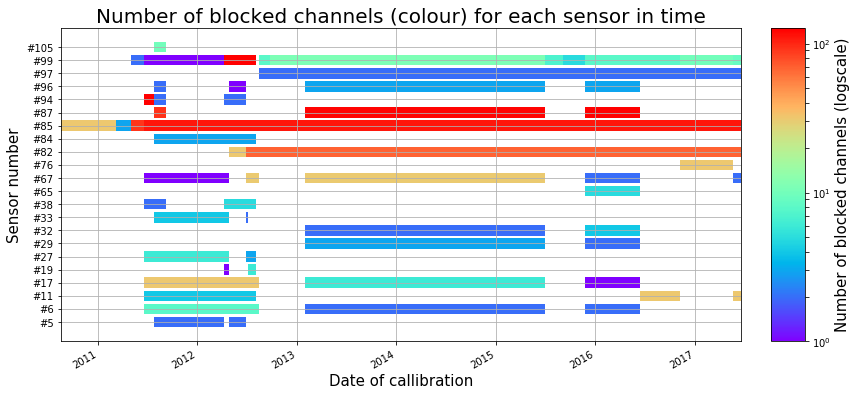
\includegraphics[width=0.7\linewidth]{figures/chapter4/calib_analysis/P3-mask-time.png}
    \caption{Distribution of blocked channels per sensor in time.}
    \label{plot:p3-mask-time}
\end{figure}

\begin{figure}
    \centering
    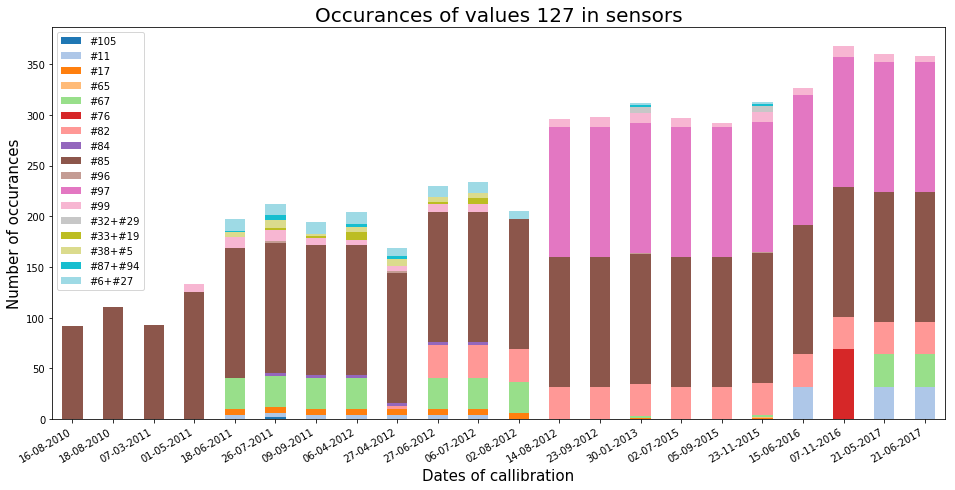
\includegraphics[width=0.7\linewidth]{figures/chapter4/calib_analysis/P3-mask-time2.png}
    \caption{Total number of occurances of masked channels versus time.}
    \label{plot:p3-mask-time2}
\end{figure}

Apart from the masked values, the usual and outlying calibration, there is still a part of the data which doesn't fit any of those categories.
This part of data can be characterised as the $H_{t} > 50 ADC \land H_{t} \neq 127 ADC$.
In the Fig \ref{plot:p3-other-outliers} depicts those other outliers. Number of occurances of these outliers change from calibration to calibration, but overall is limited to three sensors: \#85 \#67 and \#94.


\begin{figure}
    \centering
    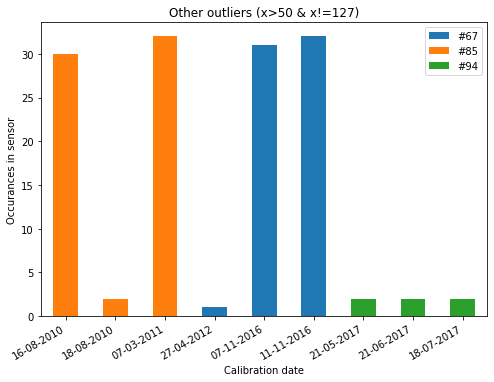
\includegraphics[width=0.7\linewidth]{figures/chapter4/calib_analysis/P3-other-outliers.png}
    \caption{Outlying values other than masked channels.}
    \label{plot:p3-other-outliers}
  \end{figure}

\section{Outlierness with probabilistic programming}
\label{chap4:outlierness}

\subsection{Dataset creation}
The analysis of the calibration data in the previous section yielded a usefule insight into the properties of the high threshold $H_t$.
A standard calibration for $R$ of $\phi$ sensor is usually close to certain value, independant of the calibration.
It is assumed that the distribution of the threshold value is given by the gaussian distribution.
The analysis of the bad (@TODO add asterisk here) calibrations shows that actually that the distribution $H_t$ is alaso dependant on the channel (e.g the regularity repeating every 500 channels).
The ``bad'' calibrations were assigned an ``outlierness'' value $X$.
This ``outlierness'' measure is purely artificial and subjectine, and also expresses a strenght of belief that a given calibration is an outlier.
The bigger the number, the stronger the belief that calibration is outlier.
There is no scale or limit on the outlierness number, other than that the 0 represents a normal calibration.
The actual assigned values can be seen in the Table \ref{data-table}.

\begin{table}[h]
\caption{\label{data-table}Outlierness calibration dataset values.}
\begin{center}
\begin{tabular}{ll}
Calibration date& X\\
2011-03-07&1\\
2012-08-02&3\\
2012-07-30&10\\
2012-08-01&10\\
all others&0\\
\end{tabular}
\end{center}
\end{table}

\subsection{Model}

For the purpose of simplicity this subsection, we will be using only the $R$-typed sensor data, and decribe a notation (@TODO linebreaks in the equation):


\begin{equation}
  \label{notation}
   T_n = H_{n}(n, R, \#, T*) \land T\prime_n = H_{n}(n, R, \#, T)
  \end{equation}

Where $n$ stands for a channel number across all sensors in time.
As mentioned previously, it is assumend that the distribution of the threshold in particular channel is gaussian.

\begin{equation}
  \label{basoc-model}
    T_n \sim Gaussian(\mu=\mu_n, \sigma=\sigma_n)
  \end{equation}

As visible in \ref{plot:only_good_all}, the value of the normal calibration for the $R $ sensor oscillates around $12 ADC$.
Therefore the parameters $\mu_{n}$ and $\sigma_{n}$ can be calculated by fitting the channels histogram to gaussian distribution.
In this case the probabilistic programming paradigm is used to achieve that. We use the dataset containing only ``good'' calibrations to calculate that.

In order to extend the model to the ``bad'' calibrations, we add additional terms to the model:

\begin{equation}
    \label{total-model}
    T\prime_n \sim Gaussian(\mu=X*\mu\prime_n+\mu_n, \sigma=X*\sigma\prime_n+\sigma_n)
\end{equation}

The $X$ stands for the outlierness of the calibration, and $\mu\prime$ and $\sigma\prime$ are coefficients of the linear dependency on the $X$.
These parameters, as previously are intrinsic property of $n$ channel.
The $X$ value is the same across given calibration date.
Notice that when the $X=0$, then, the model in Eq. \ref{total-model} is equivelent to \ref{basoc-model}.
This allows to use the parameters $\mu_{n}$ and $\sigma_{n}$ calculated for previous model, to be used in the extended one.
Given the $X$ from the \ref{data-table}, we are able to calculated $\mu\prime_{n}$ and $\sigma\prime_{n}$.

\subsection{Training}
(@TODO) add details about pymc training here

\subsection{Results}

The model presented in this subsection is a machine learning model, but is quite different from the models used frequently (such those based on neural networks).

It is not a black-box model, as for each of the channels there are only 4 parameters that are needed. Such low complexity of the model also allows for no train-test split (a usual practice in mahcine learning).
This approach has additional benefits such as:

\begin{itemize}
  \item Partial dimentional independence - This model can be used to extract the value of the outlierness not only for entire calibration, but also for a specific sensor, or module, or a group of channels, or even just specific channels. When analysing the calibration this allows for a more detailed insight as it can bring focus to a specific part of a detector that exhibits more unpredicted behaviour.
  \item Generation of artificial data - Because the probabilistic programing is based upon the statistical inference, and distributions, simply by calculating the $\mu$ and $\sigma$ parameters of gaussian distribution we are able to generate an artificial sample of the data.
  \item Interpolation and Extrapolation - This model was trained only on four different values of $X$, and yet, it is capable to asses the outlierness value not only in the range between those four values (e.g. $X=5$), but also through generation of artificial data, in can show what a calibration that this outside the scope of the data (e.g. $X=12$) might look like.
\end{itemize}

\begin{figure}
    \centering
    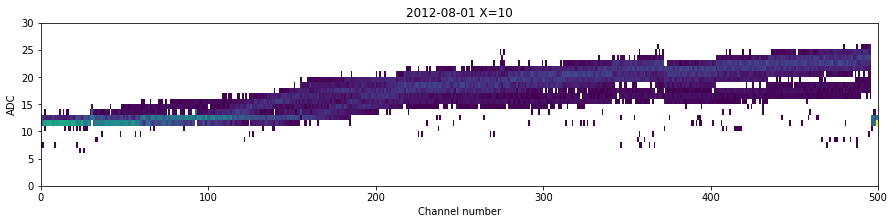
\includegraphics[width=0.7\linewidth]{figures/chapter4/outlierness/real_data.png}
    \caption{500 channels from a single calibration date marked with X=10}
    \label{plot:real-data}
  \end{figure}

\begin{figure}
    \centering
    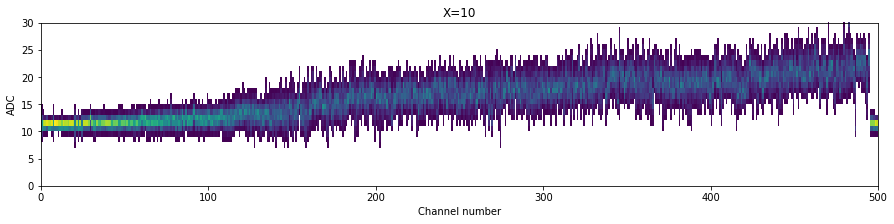
\includegraphics[width=0.7\linewidth]{figures/chapter4/outlierness/generated_data.png}
    \caption{500 channels from a single generated calibration at X=10}
    \label{plot:generated-data}
  \end{figure}

In Fig. \ref{plot:real-data} there is a sample of the data (500 chanels) that was taken of the ``bad calibrations''. It can be noted that the range of the $H_{t}$ values is on par with thos visible in the plot of the generated dataset \ref{plot:generated-data}.
(@TODO add another figure with artificial data of 12, and reference it here) Additionaly Fig there is a plot of calibration with value $X=12$, which was not present in the dataset and is actually outside the scope of the dataset.

This model was actually introduced to the Lovel monitoring system in the second half of year 2018, and was used to monitor the oncoming calibrations. The Figure \ref{plot:gui} depicts a screenshot from the monitoring system, and shows outlierness levels for the sensor \# 21. It is noticable that the value of the outlierness was slightly eleveted in 2017, which is attributed to some changes in the cooling system.


\begin{figure}
    \centering
    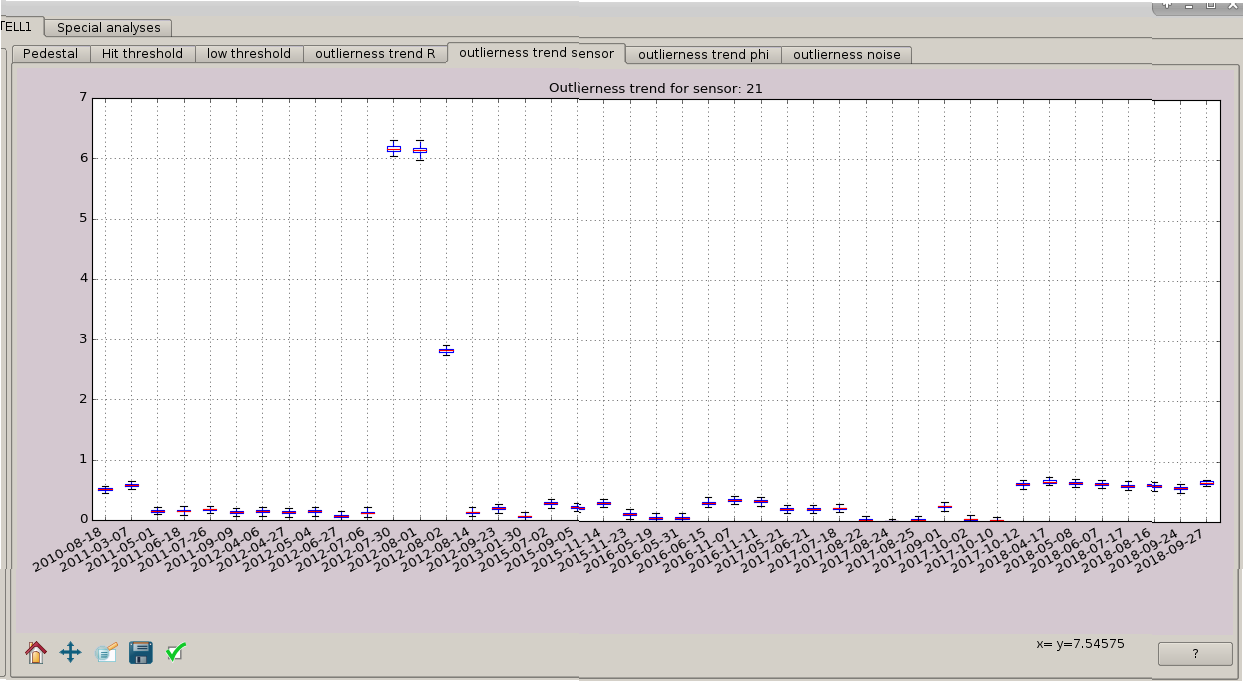
\includegraphics[width=0.7\linewidth]{figures/chapter4/outlierness/calina_lovell_screenshot.png}
    \caption{Screenshot from the outlierness monitoring in Lovell software.}
    \label{plot:gui}
  \end{figure}


\section{Dimentionality reduction}
\label{chap4:dimred}

The Velo detector in it's strip version, has 172 032 strips. Many of the parameters needed for it's calibration are calculated per strip. This is a huge amount of parameters, which is not easilly understable for human operators.
In it's pixel version, the number of such parameters will grow to 41 million (exactly $256*256*12*52 = 40894464$) \cite{Collaboration:1624070}.
Thus, an early tests of dimentionality reduction techniques will be very useful for the future. In this section we will only use high threshold parameter.
There are mutliple ways of applying PCA or autoencoder to the dataset (using different set's of values - or dimentions).
\subsection{Methods}

% @TODO explain why those two and not VAE or else
% @TODO reference the section
\subsection{Pedestals dimentionality reduction}

For the purpose of looking at what differentiates the pedestal parameter in some sensors frome the others. For this purpose we used PCA reduction, by reducing each channels time progression (a single dimentionality reduction for each of the sensor's channel).
The combined result is visible on Fig. \ref{plot:pca_pedestals_all}. Because of the high number of individual sensors, the split into several plots gives more clarity (Fig. \ref{plot:pca_all_ped}).

\begin{figure}[H]
    \centering
    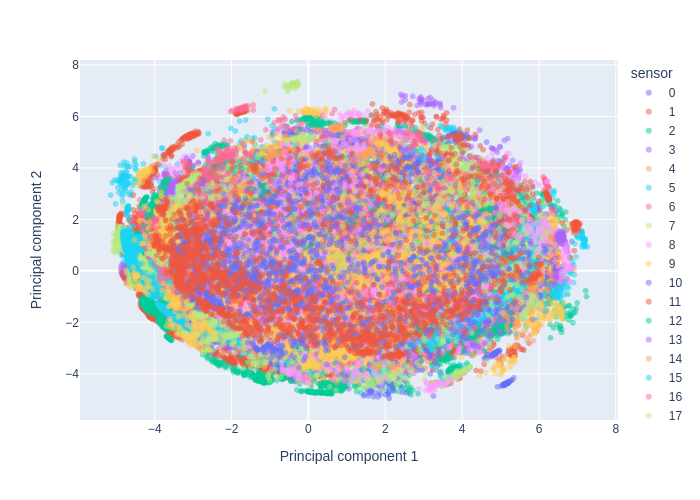
\includegraphics[width=0.7\linewidth]{figures/chapter4/dimred/PCA_pedestals_all.png}
    \caption{}
   \label{plot:pca_pedestals_all}
  \end{figure}

The reduced dataset shows a 2D gaussian distribution. It can be seen that some of the channels from a particular sensor can form clusters, or be distributed on a ring on the border of the dataset. What actually happens with a single datapoint with the tranformation can be explained by examining the particular channels. In the Fig. TODO there are 3 selected channels from a plot of the reduced data in sensor 11. Those points are also plotted at the Fig. TODO. We can see that the sensors on the opposing edges of the circle formed by the data, represent different trends in the pedestals value. Channel's 1899 pedestal value grows over time, but 543's decreases. Values in channel 322 stays high and stable. Therefore we can say that that essentially the PCA reduction separates the channels based on their trend. The 2D gaussian distribution structure makes it consistent with the trend calculation in previous sections, as the distribution centers around 0. This means that there is no overall trend (no growth, or decrease).
  
  \begin{figure}
\centering
\begin{subfigure}[b]{0.45\textwidth}
    \centering
    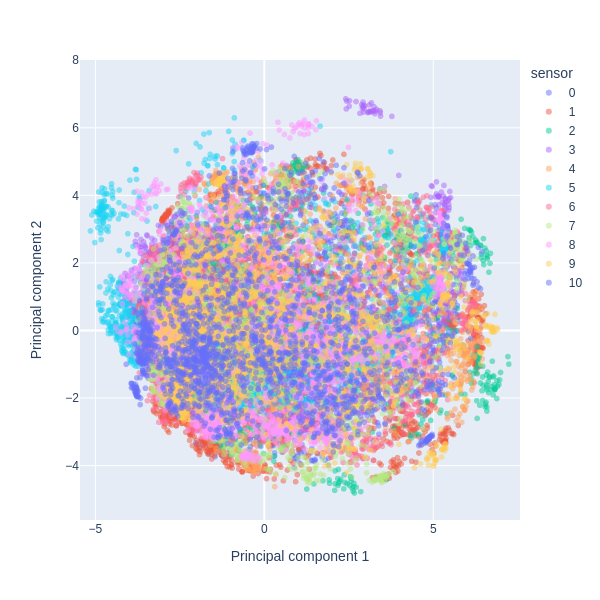
\includegraphics[width=\linewidth]{figures/chapter4/dimred/PCA_pedestals_r_phi_0.png}
\caption{PCA, R sensor type}
  \label{plot:PCA_pedestals_0}
  \end{subfigure}
\begin{subfigure}[b]{0.45\textwidth}
    \centering
    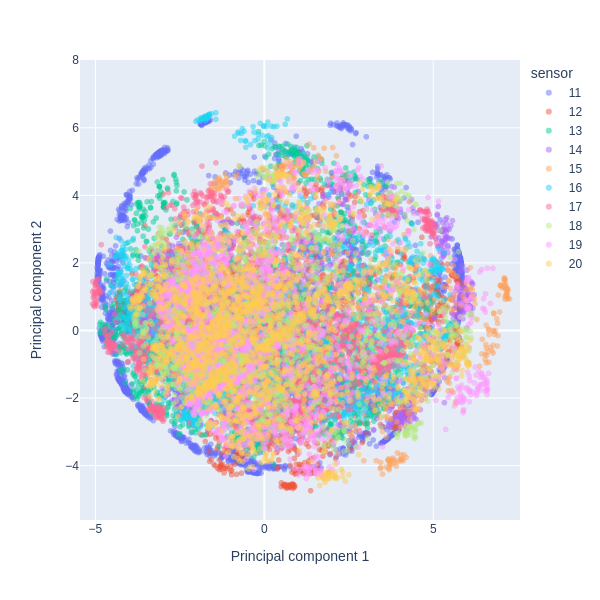
\includegraphics[width=\linewidth]{figures/chapter4/dimred/PCA_pedestals_r_phi_1.png}
\caption{PCA, phi sensor type}
   \label{plot:PCA_pedestals_1}
  \end{subfigure}


\begin{subfigure}[b]{0.45\textwidth}
    \centering
    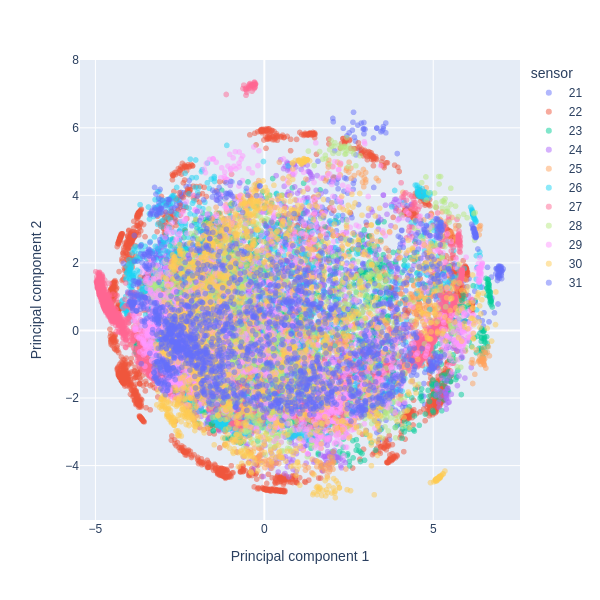
\includegraphics[width=\linewidth]{figures/chapter4/dimred/PCA_pedestals_r_phi_2.png}
% \caption{}
\caption{autoencoder, R sensor type}
    \label{plot:PCA_pedestals_2}
  \end{subfigure}
\begin{subfigure}[b]{0.45\textwidth}
    \centering
    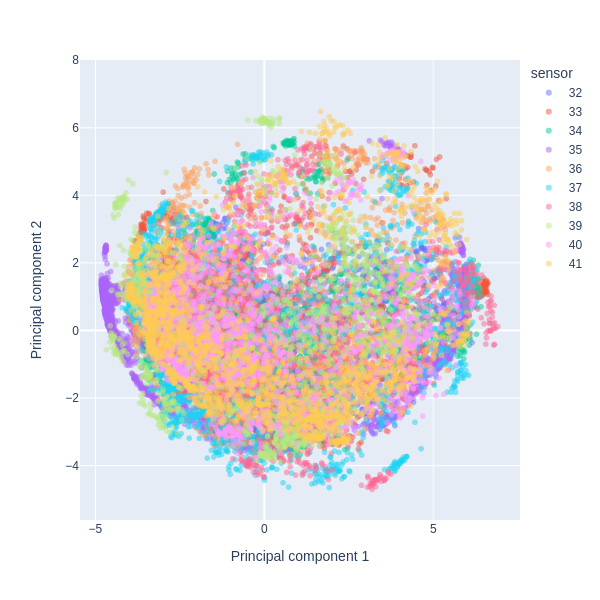
\includegraphics[width=\linewidth]{figures/chapter4/dimred/PCA_pedestals_r_phi_3.png}
\caption{autoencoder, phi sensor type}
% \caption{}
   \label{plot:PCA_pedestals_3}
  \end{subfigure}

    \caption[All calibrationd]{All of the calibrations, with reduced dimentionality using autoencoder and PCA.}
    \label{plot:pca_all_ped}
\end{figure}



 \begin{figure}
\centering
\begin{subfigure}[b]{0.45\textwidth}
    \centering
    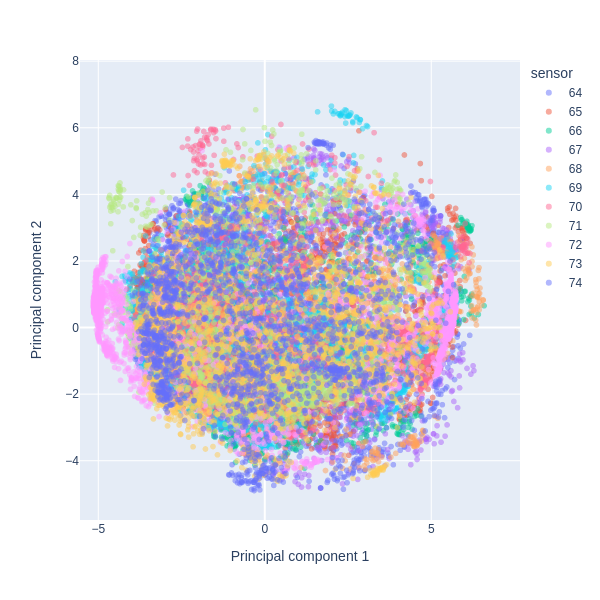
\includegraphics[width=\linewidth]{figures/chapter4/dimred/PCA_pedestals_phi_0.png}
\caption{PCA, R sensor type}
  \label{plot:PCA_pedestals_0_phi}
  \end{subfigure}
\begin{subfigure}[b]{0.45\textwidth}
    \centering
    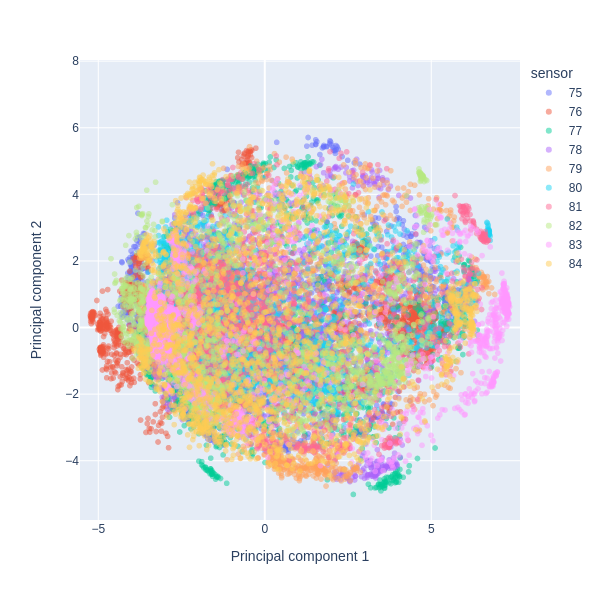
\includegraphics[width=\linewidth]{figures/chapter4/dimred/PCA_pedestals_phi_1.png}
\caption{PCA, phi sensor type}
   \label{plot:PCA_pedestals_1_phi}
  \end{subfigure}


\begin{subfigure}[b]{0.45\textwidth}
    \centering
    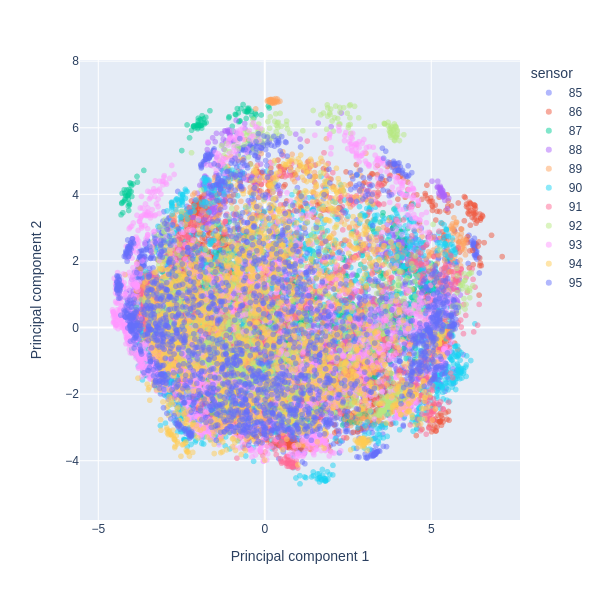
\includegraphics[width=\linewidth]{figures/chapter4/dimred/PCA_pedestals_phi_2.png}
% \caption{}
\caption{autoencoder, R sensor type}
    \label{plot:PCA_pedestals_2_phi}
  \end{subfigure}
\begin{subfigure}[b]{0.45\textwidth}
    \centering
    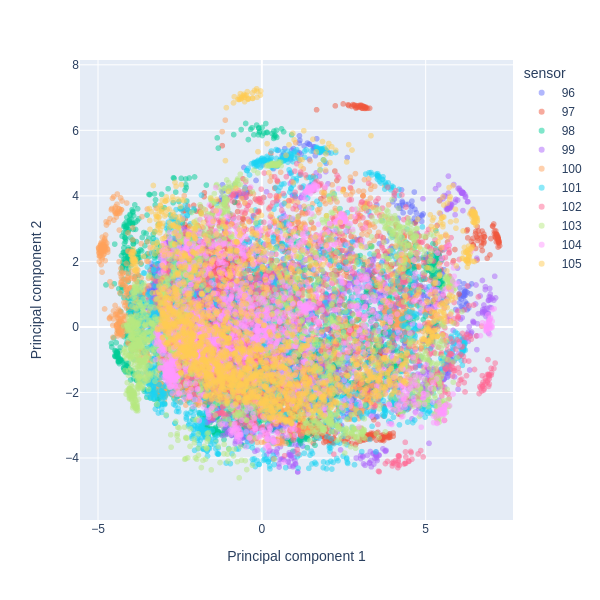
\includegraphics[width=\linewidth]{figures/chapter4/dimred/PCA_pedestals_phi_3.png}
\caption{autoencoder, phi sensor type}
% \caption{}
   \label{plot:PCA_pedestals_3_phi}
  \end{subfigure}

    \caption[All calibrationd]{All of the calibrations, with reduced dimentionality using autoencoder and PCA.}
    \label{plot:pca_all_ped_phi}
\end{figure}


\begin{figure}
    \centering
    
    \begin{subfigure}[b]{.5\textwidth}
    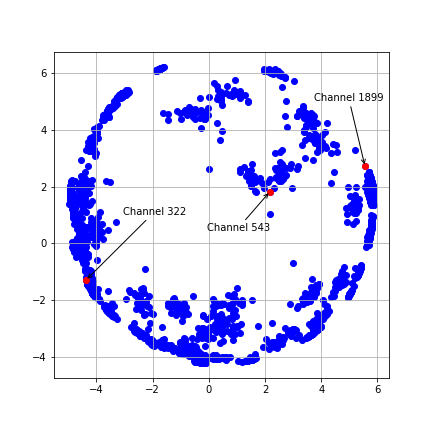
\includegraphics[width=\linewidth]{figures/chapter4/dimred/selected_channels_ped.png}
    \caption{ .}
   \label{plot:PCA_selected}
  \end{subfigure}\begin{subfigure}[b]{.5\textwidth}
    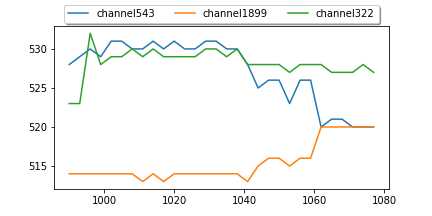
\includegraphics[width=\linewidth]{figures/chapter4/dimred/PCA_trends_channel.png}
    \caption{ .}
   \label{plot:PCA_trend}
  \end{subfigure}
      \caption[All calond]{All of the calibrations, with reduced dimentionality using autoencoder and PCA.}
    \label{plot:pca_all}
  
  \end{figure}





\subsection{Threshold dimentionality reduction}


The most usefult is feeding the algorithm with each of the sensors, with separation for the R and phi types of sensors.
This allows us to easilly see changes common for all of the sensor at once.
In Figures \ref{plot:pca_progression_r}-\ref{plot:nn_progression_phi}, you can see ten consecutive calibrations plotted after dimentionality reduction of a single sensor ($n_{dim}=2048$) to a 2D ($n_{dim}=2$), and plotted on a plane.
The color represents the number of a sensor.
In both of the plots made using PCA and autoencoders you can see that two outlying dates (2012-07-30 and 2012-08-01) stand out significantly.
In contrast with autoencoder, the PCA is deterministic, and does not require random initialisation. Because of this, there may be some variance in autoencoder model results, even when using exactly the same setup.

% \ref{plot:pca_progression_r},  \ref{plot:pca_progression_phi}, \ref{plot:nn_progression_r}, \ref{plot:nn_progression_phi},

\begin{figure}[H]
    \centering
    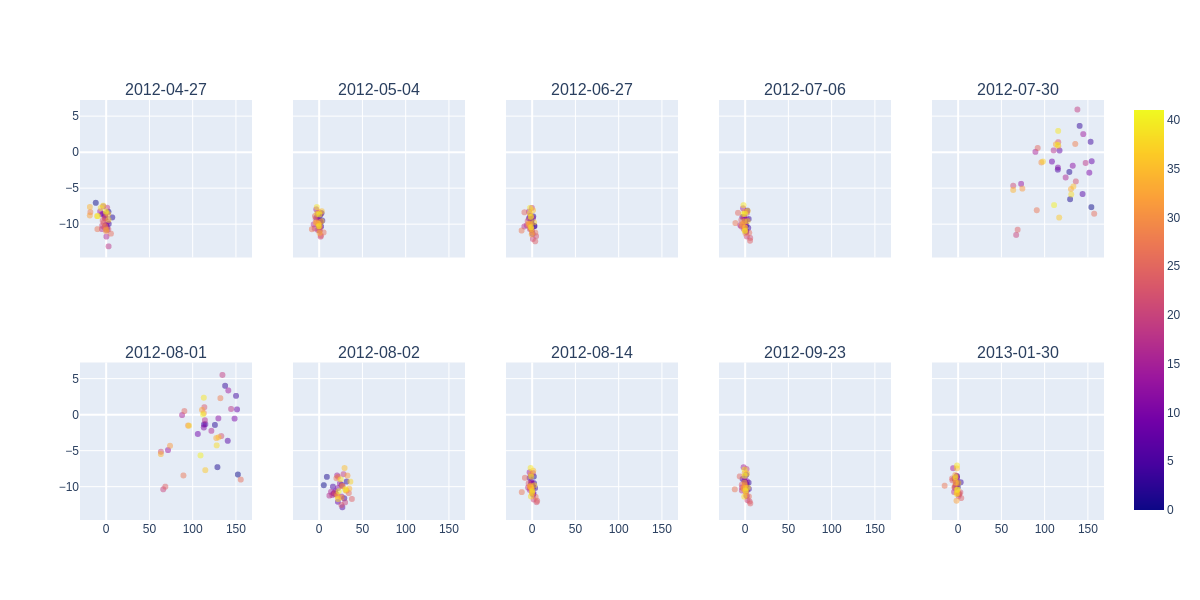
\includegraphics[width=\linewidth]{figures/chapter4/dimred/PCA_module_R_together.png}
    \caption{Time progression of selected section of calibration dates, with reduced dimentionality using PCA, only for R sensors.}
   \label{plot:pca_progression_phi}
  \end{figure}

\begin{figure}[H]
    \centering
    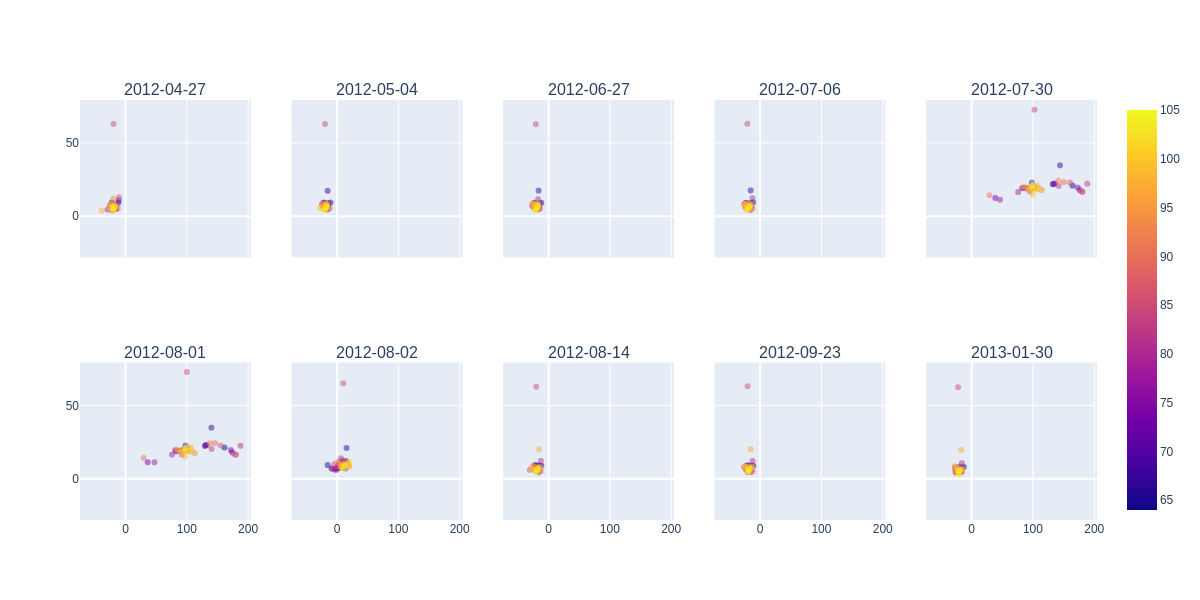
\includegraphics[width=\linewidth]{figures/chapter4/dimred/PCA_module_phi_together.png}
    \caption{Time progression of selected section of calibration dates, with reduced dimentionality using PCA, only for phi sensors.}
   \label{plot:pca_progression_r}
  \end{figure}

\begin{figure}[H]
    \centering
    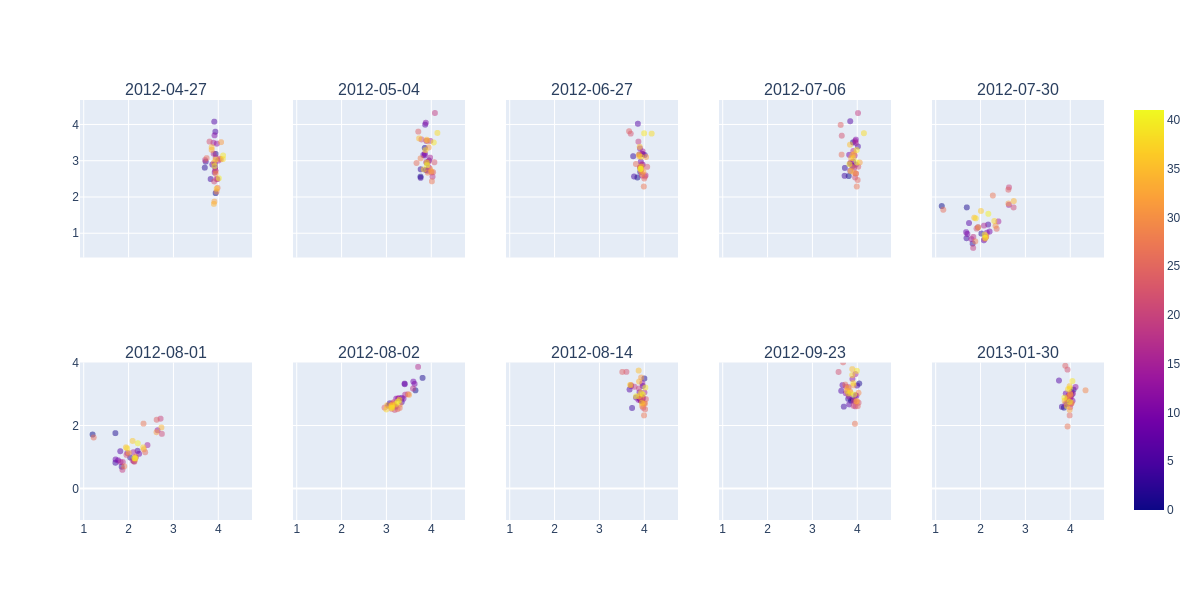
\includegraphics[width=\linewidth]{figures/chapter4/dimred/NN_module_R_together.png}
    \caption{Time progression of selected section of calibration dates, with reduced dimentionality using autoencoder, only for R sensors.}
   \label{plot:nn_progression_r}
  \end{figure}

\begin{figure}[H]
    \centering
    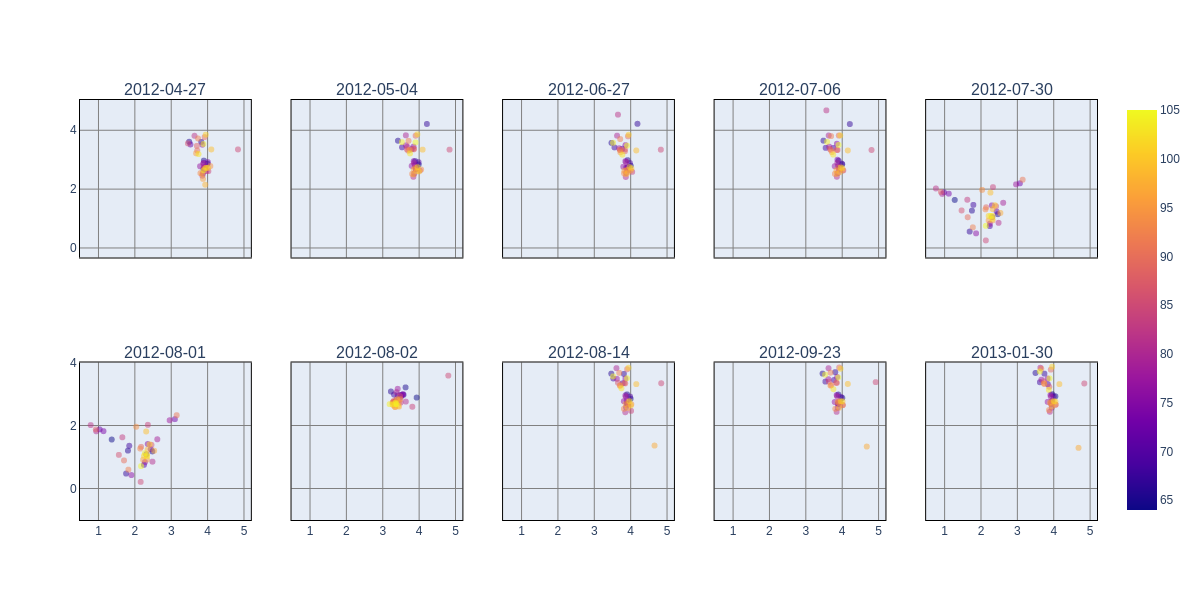
\includegraphics[width=\linewidth]{figures/chapter4/dimred/NN_module_phi_together.png}
    \caption{Time progression of selected section of calibration dates, with reduced dimentionality using autoencoder, only for phi sensors.}
   \label{plot:nn_progression_phi}
  \end{figure}

  The Figures \ref{plot:pca_all_r}-\ref{plot:nn_all_phi} represent all calibration dates on the same plot, splitted into different sensors, and created with different techniques. Notice that all of the plots have different scales of the axes, as the methods used to reduce dimentionality do not retain the scale. The most useful insight to those plots is that the relative change represents outlying calibrations.

\begin{figure}
\centering
\begin{subfigure}[b]{0.45\textwidth}
    \centering
    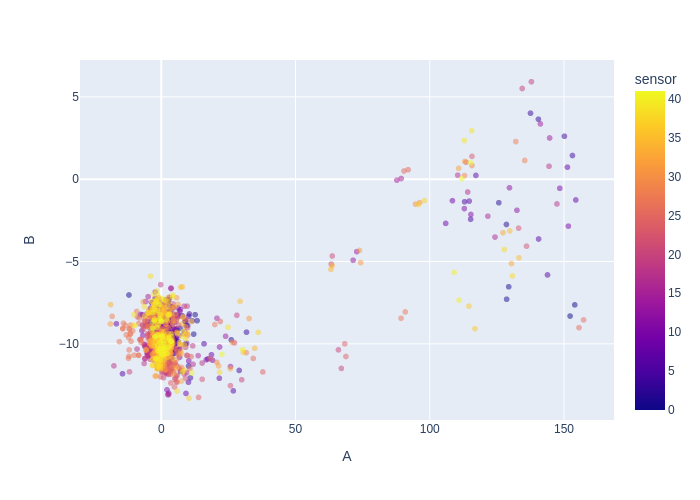
\includegraphics[width=\linewidth]{figures/chapter4/dimred/PCA_module_R_all.png}
\caption{PCA, R sensor type}
   \label{plot:pca_all_r}
  \end{subfigure}
\begin{subfigure}[b]{0.45\textwidth}
    \centering
    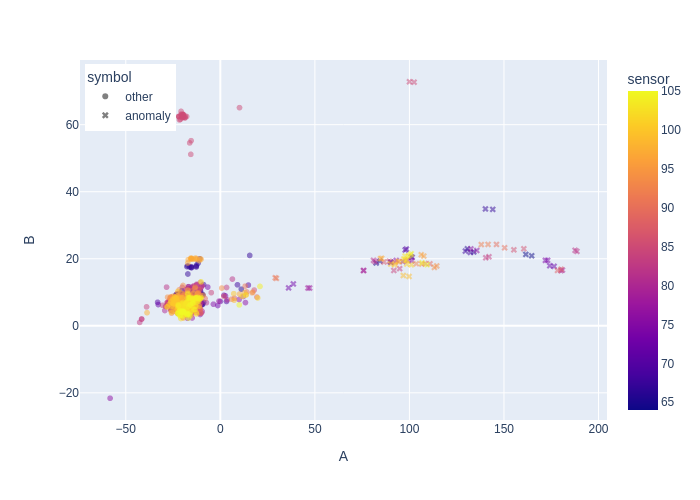
\includegraphics[width=\linewidth]{figures/chapter4/dimred/PCA_module_phi_all.png}
\caption{PCA, phi sensor type}
   \label{plot:pca_all_phi}
  \end{subfigure}


\begin{subfigure}[b]{0.45\textwidth}
    \centering
    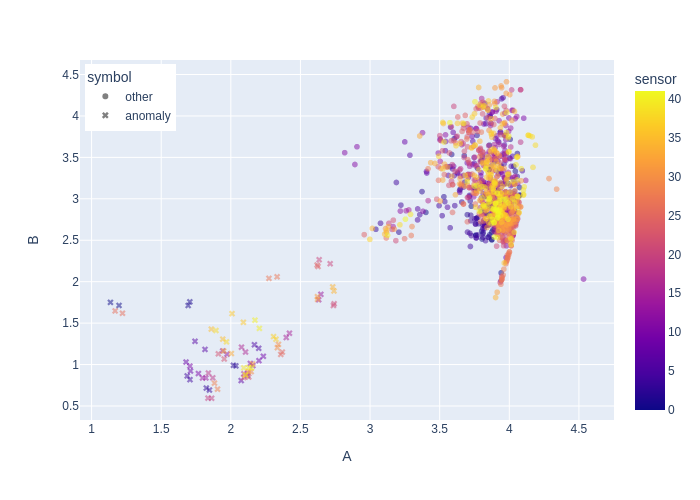
\includegraphics[width=\linewidth]{figures/chapter4/dimred/NN_module_R_all.png}
% \caption{}
\caption{autoencoder, R sensor type}
   \label{plot:nn_all_r}
  \end{subfigure}
\begin{subfigure}[b]{0.45\textwidth}
    \centering
    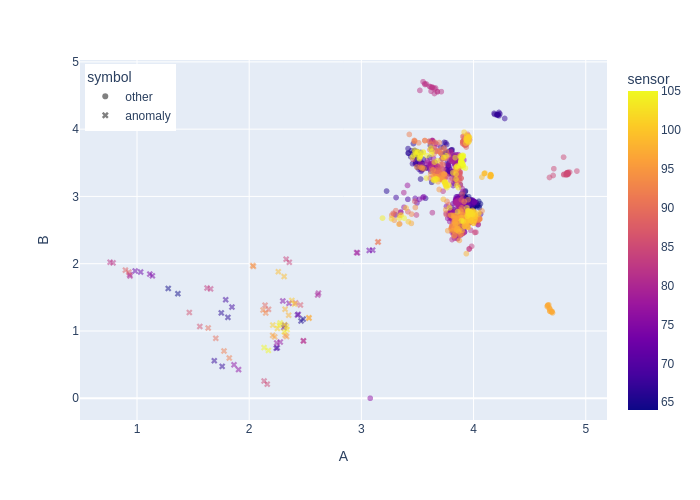
\includegraphics[width=\linewidth]{figures/chapter4/dimred/NN_module_phi_all.png}
\caption{autoencoder, phi sensor type}
% \caption{}
   \label{plot:nn_all_phi}
  \end{subfigure}

    \caption[All calibrationd]{All of the calibrations, with reduced dimentionality using autoencoder and PCA.}
\end{figure}
\section{Time to calibration forecasting}
\label{chap4:wtte}
The calibration of the detector is essential for it's proper use. It set's all of the parameters of the detector that will be needed during the data taking.
In Velo runs 1 and 2 of the LHC it was possible that if the channel thresholds were set too high, useful data could be lost. When a electrical signal coming from a single strip would not exceed the threshold, it would be discarded.
Therefore it is crutial for the detector operations to have as frequent calibrations as possible.
But the calibration process requires a noise data recorded when there is no beam present. Ideally, the longer the time that it takes to record the noise, the better the callibration accuracy (gaussian noise mean calculation. This also means that calibration requires a special time slot in between data taking, when no beam is present.
This motivates the studies of the forecasting of the need for calibration in Velo.

\section{Dataset}
In the data availible to the analysis we can distinguish two kinds of data: raw data and calibration data.
The raw data is the data that is recorded during the beam conditions, and the calibration data is the data taken during no-beam.
The actual way of calculating the values present in the data does not differ.
%@TODO reference the data analysis
\begin{figure}
    \centering
    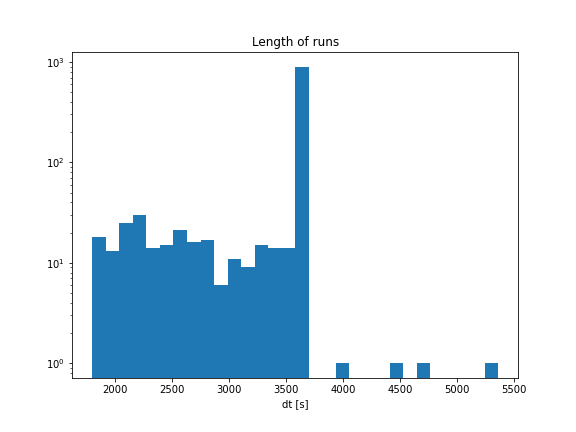
\includegraphics[width=0.6\linewidth]{figures/chapter4/wtte/runlengths.png}
    \caption{Histogram of lengths of runs in the dataset, expressed in seconds. Significant ammount of runs lasted about 3600 seconds (1 hour).}
    \label{plot:runlen}
  \end{figure}
The ammount of datapoints is significantly greater for the raw data, as it was taken in any single data run, which can last from a few seconds, to about an hour.
Calibration data on the other hand was taken every few weeks.
In both kinds of the data there is a constant dimentionality of the parameters, as each of the values was taken for each of the 2048 channels of the sensor individually, in total giving a 172 032 values of a single parameter for the whole detector.
The analysis of the trends of the trends has produced a candidate for a parameter that could be used to identify a need for a calibration.
The \textit{pedestal subtracted} $\Delta\mu$  parameter is the value of the mean of the noise calculated as follows:
\begin{equation}
    \Delta\mu = \mu_{current} - \mu_{calibration}
\end{equation}
Where $\mu_{current}$ is mean of the signal coming from the current run.
The analysis of this parameter has shown that a value of the standard distribution of this paremeter $\sigma(\Delta\mu)$ within the detector grows after the calibration, and drops after one.
An example of this is present at the \ref{plot:wtte1-stdevs}.
\begin{figure}
\centering
\begin{subfigure}[b]{0.85\textwidth}
    \centering
    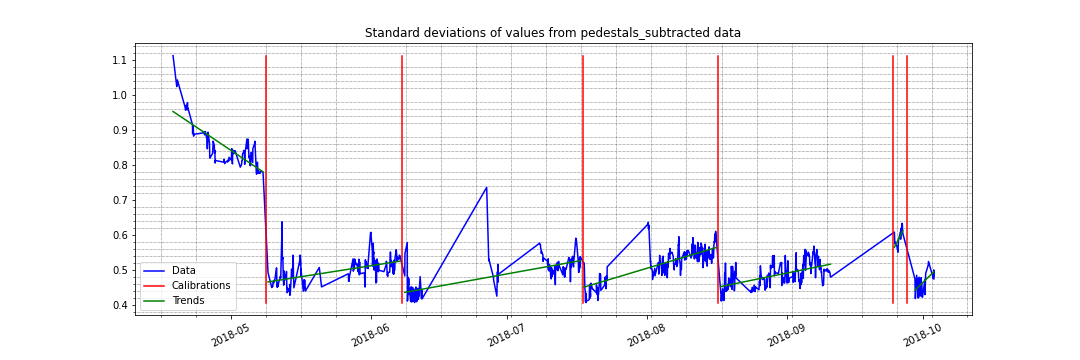
\includegraphics[width=\linewidth]{figures/chapter4/wtte/stdevs_trends_calibs.png}
% \caption{}
    \label{plot:wtte1-stdevs}
  \end{subfigure}

\begin{subfigure}[b]{0.85\textwidth}
    \centering
    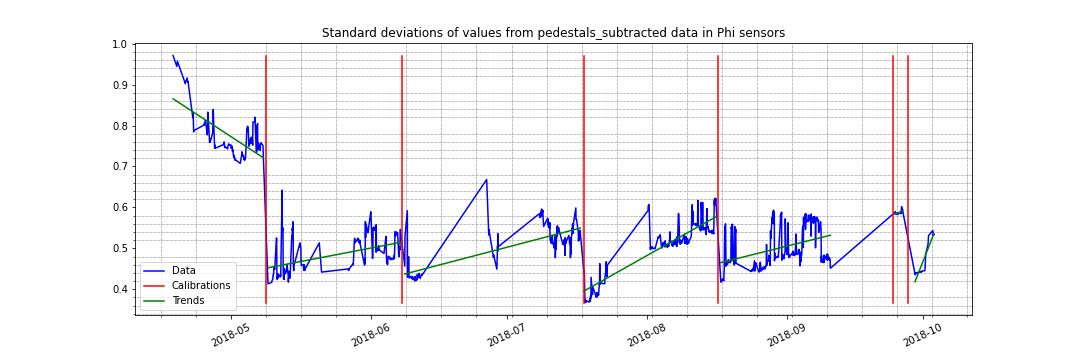
\includegraphics[width=\linewidth]{figures/chapter4/wtte/pstdevs_trends_calibs.png}
% \caption{}
    \label{plot:wtte1-p-stdevs}
  \end{subfigure}

\begin{subfigure}[b]{0.85\textwidth}
    \centering
    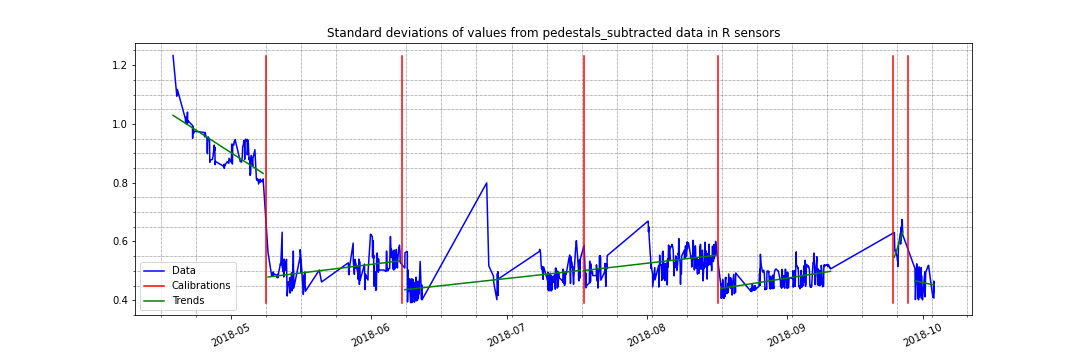
\includegraphics[width=\linewidth]{figures/chapter4/wtte/rstdevs_trends_calibs.png}
% \caption{}
    \label{plot:wtte1-r-stdevs}
  \end{subfigure}
  \caption[Two numerical solutions]{ Standard deviation of the pedestal subtracted parameters in the whole sensor (top), pedestal subtracted in Phi sensors (middle), and in R sensors (bottom).
  Calibration dates are in red, and the green lines present trends calculated between calibrations.}
\end{figure}

% @TODO add image reference.

The data used for the forecasting model comes from 2018. The calibration process and raw data in 2018 is a best candidate because of the frequently occuring runs, and calibrations. The exact timespan of the data is from 2018-05-08 to 2018-09-24.
This constitues exactly 4 calibration periods. The used data comes in a form of $\sigma(\Delta\mu)_{t}$ where $t$ stands for a given run time.
The time information is translated to delta time ($dt_{n} = t_{n}-t_{n-1}$). The continious time series of data is processed to a windowed time-series, of 100 data points, beginning with the first data point after calibration, and padded with zeroes.

% @TODO show an examplary data
%

\begin{equation}
X_{it} = \begin{bmatrix} std_{it} \\ dt_{t} \end{bmatrix}
\end{equation}

As it is a case of supervised learning, the additional component $Y_{it}$ is set to be a number of days left until next calibration. We have chosen the number of days as the most suitable time range for this purpose, as there can be many runs per day,

% @TODO why not an exact time ?

\section{WTTE-RNN for Velo}


% @TODO reference the discussion of wtte-rnn
% @TODO explain why wtte-rnn

The WTTE-RNN as discussed in Sec ... is a one layer capable of outputing the parameters of the weibull distribution. The actual type of a problem in machine learning is called survival analysis, architecture of the neural network used for forecasting is present at the Table \ref{tab:network}. It contains 6 layers in total. The LSTM layer is necessary for the time series that is used as input data.

\begin{table}[h]
% https://app.neptune.ai/mmajewsk/wtte-calib/e/WTTEC-83/source-code?path=source_code&file=dense_module.py&attribute=files&filePath=.
\begin{center}
\begin{tabular}{ |c|c|c| }
\hline
Layer No. & Layer type & Layer size\\
\hline
1 & Dense & 43\\
2 & Dropout & \\
3 & LSTM & 20\\
4 & Activation - Tanh & \\
5 & Dense & 2\\
6 & WTTE-Activation & \\
\hline
\end{tabular}
\caption{\label{tab:network}The neural network layers used for the WTTE-RNN model}
\end{center}
\end{table}



\section{Mask clustering}

The VeloPix masks flags are veru useful things. They help to spot if there is something wrong with the detector.
%@TODO explain here where does the masks come from 
%@TODO explain here how come there are clusters in masks

The cluster masks can pose a threat to the reconstruction algorithm, and the radial reconstruction resolution.
As such they have to be monitored. 
\subsection{Mask simulation}

Due to the VeloPix being still under developement and comissioning during these studies, the experience gained with the tests of VeloPix was used to create a simulation of occuring masks.

%@TODO insert mask picture here

In order to make a realistic simulation we have used a process consisting of three types of intrusions:

\begin{itemize}
  \item Random uniform changes $P$, in which a random portion of pixels changes their state to masked
  \item Linear cluster $L$ where a linear portion of pixels are masked.
  \item Blob cluster $G$ with masks created by a 2D isotropic gaussian distribution.
\end{itemize}

These intrusions are added to an initially empty matrix with a different probabilities. Each of the intrusions is created on a empty matrix with the same size as the sensor, and is simply added to the simulated matrix $M$.
One crutial step of this simulation is random cleaning of the matrix, in which random 80\% of the pixels are unset to a non-mask state.
The pseudocode can be found in listing \ref{alg:two}.
This process creates a continious simulation of a VeloPix matrix masks, as the new masks and clusters are generated, and the old ones slowly dissappear.


%@TODO images !!!

\SetKwComment{Comment}{/* }{ */}

\begin{algorithm}[H]
\caption{An algorithm with caption}\label{alg:two}
\KwData{$n \geq 0$}
\KwResult{$y = x^n$}
$N \gets n$\;
\While{$N \neq 0$}{
  \uIf{random() $< blob\_prob $ }{
    $M \gets M + G$
  }
  \uElseIf{random() $< line\_prob $ }{
    $M \gets M + L$
  }
    \Else{$M \gets M + P$}
    $M \gets M + Pu$
    
    $N \gets N - 1$
}
\end{algorithm}




\subsection{Clustering}

There are many clustering algorithms present in the field of machine learning. Although they all come under the term "clustering" there are actually multiple different goals that can be achieved by different algorithms. The most common density search clustering algorithms are DBSCAN and OPTICS. The details of these algorithms are described in section \ref{sec:clustering}.
In the case of application of the clustering algorithm towards masks in calibration, the desired algorithm should be able to
%@TODO mention that clustering in this case does not mean to cluster all of the point on te matrix

\begin{figure}[h]
\centering
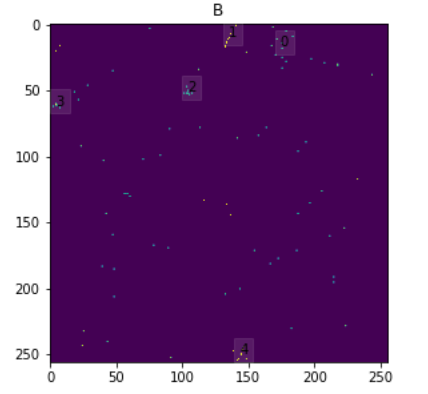
\includegraphics[width=0.5\textwidth]{figures/chapter4/velopix_clusters/dbscan_clusters.png}
\caption{And examplary clusterisation using DBSCAN ($\epsilon$ = 10, MinPts = 4) on the binary pixel-map. Clusters are numbered 1-5.}
\label{fig:dbscan_clusters}
\end{figure}

\subsection{Cluster features}

After finding the individual clusters on one calibration (a one set of masks), the clusters of masks can be characterised by a set of features.
\begin{enumerate}
\item \textbf{Position}  {$p_k$ = ($\bar{x_k}$, $\bar{y_k}$}), where $\bar{x_k} = \frac{\sum_{i}^{N^k}x_k^i}{N_k},
    \bar{y_k} = \frac{\sum_{i}^{N^k}y_k^i}{N_k}$.
\item \textbf{Size} $s_k$ = \{$n_k$, $d_k$\} where $n_k$ is the number of pixels in a cluster divided by the mean number of the pixels in the given sensor's clusters.
\item \textbf{Shape} $h_k$ = \{$\alpha_k$, $c_k$\}, where $\alpha_k$ is the directional coefficient of the cluster measured by the fit to the line $y^k(x) = \alpha_k*x + b_k$. The $c_k$ is the roundness of the cluster calculated as it's Pearson Coefficient.
\end{enumerate}
With those metrics, we can then define the spacial charecteristic vector as $v_k = [s_k; h_k]$. Then we define cluster as a set of unique features $cluster_k = {p_k, v_k}$.

\subsection{Cluster tracking}

This set of unique features is used to characterise every cluster found in the calibration.
The $cluster_{k}$ features are then used to identify cluster $k$ from timestep $t_{n}$ as te same in the timestep $t_{n-1}$.
It is performed by calculating a cosine similarity matrix $M$. The $M$ matrix is calculated in the following manner:

\begin{equation}
    M_{i,j} = \Phi_{i,j} * V_{i,j}
\end{equation}

Where $\Phi$ is defined as:
\begin{equation}
    \Phi_{i,j} = \frac{1}{d_{min}}*\max(d_{min} - D_{i,j}, 0)
\end{equation}

and $ D_{i,j} $ is a distance matrix:
 \begin{equation}D_{i,j} = || p_j - p_i ||\end{equation}

The value $d_{min}$ is set to be a limiting factor. If the distance of centroids of the clusters stays the same, the value is 1., but as the distance approaches $d_{min}$ the value approaches 0.
In the tests of the cluster tracking $d_{min}=10$ was used.
Exemplary pairing of the clusters in consecutive simulation steps is visible in the Fig. \ref{fig:fin_clus} with it's simmilarity matrix calculation in \ref{fig:sims}.

\begin{figure}[h]
\centering
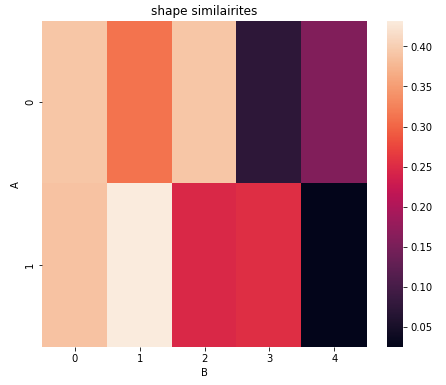
\includegraphics[width=0.3\textwidth]{figures/chapter4/velopix_clusters/shape.png}
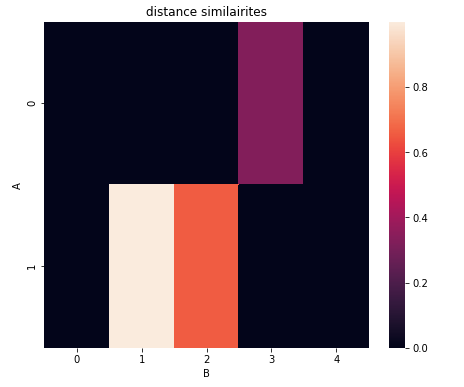
\includegraphics[width=0.3\textwidth]{figures/chapter4/velopix_clusters/distance.png}
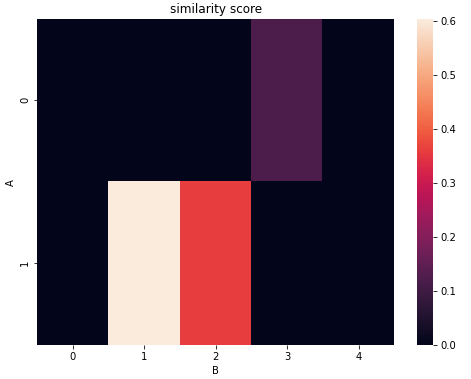
\includegraphics[width=0.3\textwidth]{figures/chapter4/velopix_clusters/similarity.png}
\caption{Rows represent clusters on image A in Figure ~\ref{fig:fin_clus}, columns represent clusters on image B in Figure ~\ref{fig:fin_clus}. Values indicate the Spacial Characteristics Similarity Measure \textit{V} (left plot), and Positional Similarity Measure \textit{$\Phi$} (middle plot). The M matrix is the rightmost plot.
}
\label{fig:sims}
\end{figure}



\begin{figure}[H]
\centering
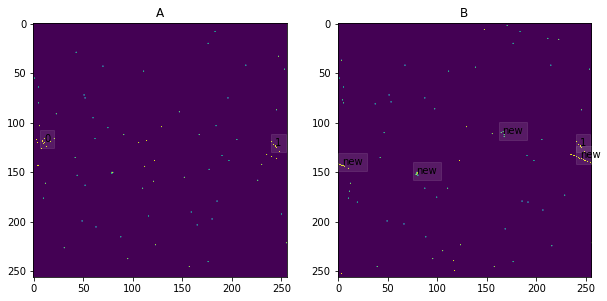
\includegraphics[width=0.7\textwidth]{figures/chapter4/velopix_clusters/paired.png}
\caption{Clusters labelled with the same integer are chosen by the algorithm as the consecutive generations of the same cluster. Clusters labeled as 'new' are clusters on the time step $t_{n}$ that were absent on time step $t_{n-1}$.}
\label{fig:fin_clus}
\end{figure}

 \subsection{Results}


The DBSCAN and OPTICS algorithms were tested on the 3000 consecutive steps of simulation of a single sensor.
The ground truth in context of clustering of the masks is not something that can v determined in the real world data.
But the simulation along with the simulation steps, can attribute any generated mask pixel to it's source (random uniform, linear, gaussian blob), thus providing information that can be used as ground truth.
It is assumed that the generated pixel should be identified as belonging to a cluster after up to 8 timesteps.
The Table \ref{sample-table} presents a confusion matrix calculated using that ground truth information. The OPTICS algorithm has three more times as many false positives as the DBSCAN. On the other hand it has almost twice more true positives.


\begin{table}[H]
  \caption{Confusion matrix values in 3000 consecutive simulation steps.}
  \label{sample-table}
  \centering
  \begin{tabular}{lll}


    \toprule
    Value     & OPTICS     & DBSCAN \\
    \midrule
    True Negative & 7608 & 16207 \\
    False Positive    & 11680 & 3081      \\
    False Negative     & 1156       & 3167  \\
    True Positive &  5665 &   3654   \\
    \midrule
    Accuracy &  0.51 &   0.76   \\
    Precision &  0.33 &   0.54   \\
    \bottomrule

  \end{tabular}
\end{table}

Both algorithms have been tested towards the ability to track the consecutive cluster's pixels through the steps of the simulation. Fig. \ref{fig:decay} depicts the number of the masks assosiated with any cluster starting at the timestep of introduction of said masked pixel. It is clearly visible that The OPTICS algorithm recognises more pixels as belonging to clusters, and for extended ammount of time, whereas the DBSCAN very quickly drops it's attention to the pixels.

\begin{figure}[H]
\centering
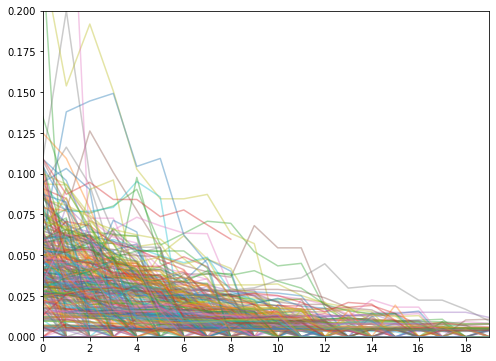
\includegraphics[width=0.4\textwidth]{figures/chapter4/velopix_clusters/optics_decay.png}
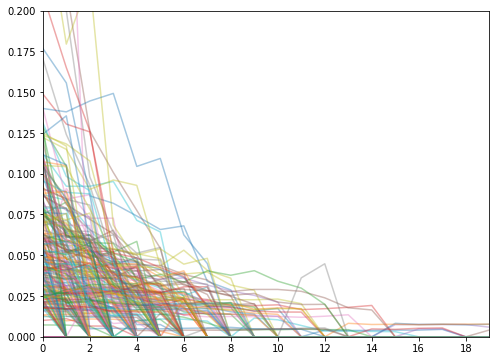
\includegraphics[width=0.4\textwidth]{figures/chapter4/velopix_clusters/dbscan_decay.png}
\caption{The fraction of pixels categorised as belonging to any clusters (Y axis) in next consecutive calibrations (X axis), since the cluster introduction to calibration (number of timesteps $n=300$). The number of detected pixels slowly decreases with time. The OPTICS algorithm (left plot) recognises the pixels of the clusters as belonging to a cluster (not necessarily the same one) for a longer amount of time. The DBSCAN is more strict in distinguishing the pixels that belong to clusters.
}
\label{fig:decay}
\end{figure}

The important test is the influence of the clustering algorithm towards the cluster tracking ability. The Fig. \ref{fig:progress} shows total number of clusters in given timestep of a simulation, being recognised as new, or retaining from previous timestep. It is clear that the cluster tracking with OPTICS detects much more clusters as new, and looses more clusters from callibration to callibration, whereas the DBSCAN, if finding less new clusters, and retaining old ones.

\begin{figure}[H]
\centering
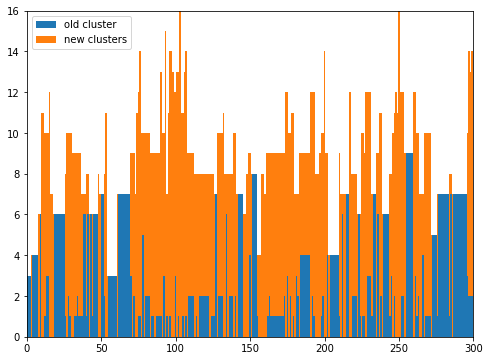
\includegraphics[width=0.4\textwidth]{figures/chapter4/velopix_clusters/optics_progress.png}
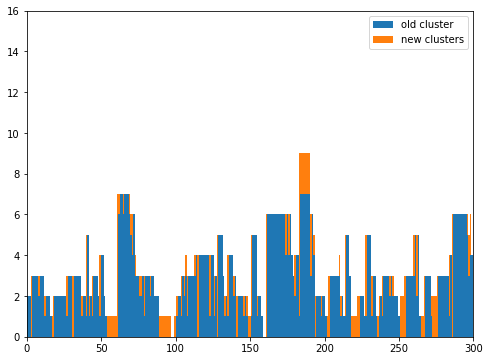
\includegraphics[width=0.4\textwidth]{figures/chapter4/velopix_clusters/dbscan_progress.png}
\caption{ The number of clusters classified as being "old" - same as in previous calibration (blue colour), and a number of clusters marked as "new" - not being the same clusters as in previous calibration (orange color). The left plot belongs to OPTICS, and the one on the right to DBSCAN.
}
\label{fig:progress}
\end{figure}

\section{Studies of surrogate function in VeloPix}

(@TODO add something here)
\subsection{Surrogate function}

(@TODO add something about how the surrogate functions works, that there is somne charge created at the sensors to calibrate)
The surrogate function is the function that relates the TOT count to the charge gathered in the VeloPix pixel \cite{Tsopelas:2016cjb}.
It has the following structur:

% \begin{equation}
%   \label{eq:surrogate}
%   ToT(q) = g \dot q + ToT_{0} - \frac{c}{q-t} + o
%   \end{equation}


\begin{equation}
  \label{eq:surrogate}
  ToT(q) = p_{0} + p_{1} \dot q - \frac{c}{q-t}
  \end{equation}
It has four free parameters: $p_{0},p_{1},c,t$, and is essentially a convolution of linear and hyperbolic functions. There is existings underlying assumption that $q > 0$.
An examplary surrogate function is visible on \ref{fig:surrogate} (@TODO explain that plot better)


\begin{figure}[H]
\centering
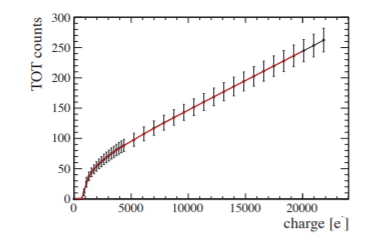
\includegraphics[width=0.7\textwidth]{figures/chapter4/surrogates/surrogate_example.png}
\caption{An examplary plot of surrogate funciton.}
\label{fig:surrogate}
\end{figure}

\subsection{Dataset}

This analysis uses the dataset gathered during the testbeam phase of the Velopix.
(@TODO explaine the testbeam here)
(@TODO explain the sensor markings here)

\subsection{Cross sensor study}
The test beam data contained multiple different types of sensors, with different types of irradiation.
Unfortunately, in the entire datsaet, there is only one sensor that is suitable for the studies of surrogates in function of fluence.
This is due to the irradiation profile of the sensors. Sensor s8 was the only one that had a clear, non-uniform profile of the irradiation, that allowed for a binning of the sensor based on the ammount of irradiation that the sensors were exposed to.

nonetheless we investigate other sensors and their distribution of the parameters in the Fig. \ref{fig:sensor_surrogate_p1}  and \ref{fig:sensor_surrogate_p2}.
The important insight is that for most of the sensors, the overall distribution post irradiation moved to the left for the $p0$ and $p1$.
For the parameters $c$ and $t$ the trend is not as obvious, and we will explain the further analysis.


\begin{figure}
\centering
\begin{subfigure}[H]{0.85\textwidth}
    \centering
    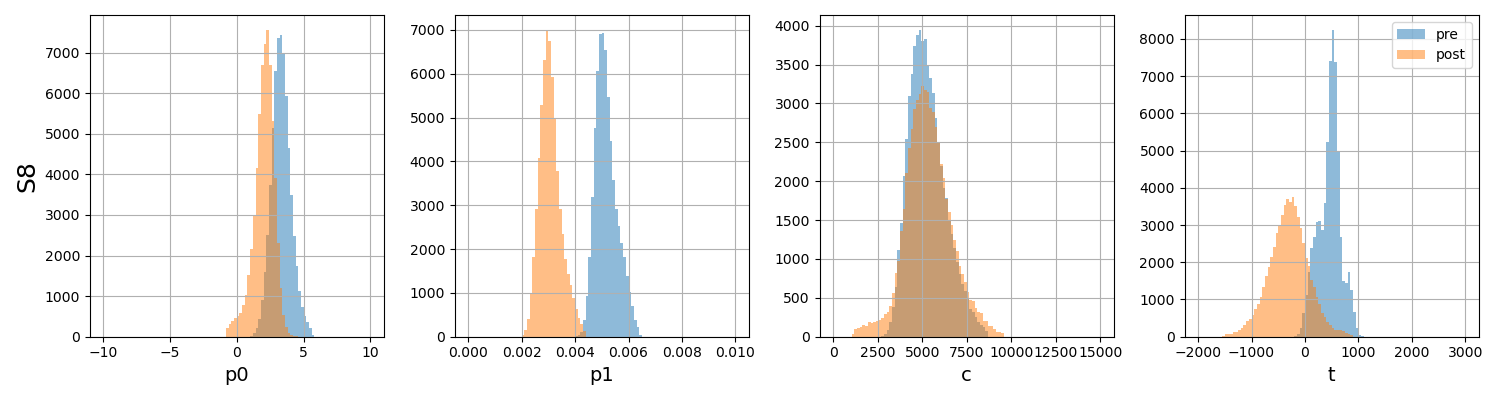
\includegraphics[width=\linewidth]{figures/chapter4/surrogates/p1_S8_histos.png}
% \caption{}
    % \label{plot:wtte1-stdevs}
  \end{subfigure}

\begin{subfigure}[b]{0.85\textwidth}
    \centering
    \includegraphics[width=\linewidth]{figures/chapter4/surrogates/p1_S16_histos.png}
% \caption{}
    % \label{plot:wtte1-stdevs}
  \end{subfigure}

\begin{subfigure}[b]{0.85\textwidth}
    \centering
    \includegraphics[width=\linewidth]{figures/chapter4/surrogates/p1_S17_histos.png}
% \caption{}
    % \label{plot:wtte1-stdevs}
  \end{subfigure}

\begin{subfigure}[b]{0.85\textwidth}
    \centering
    \includegraphics[width=\linewidth]{figures/chapter4/surrogates/p1_S21_histos.png}
% \caption{}
    % \label{plot:wtte1-stdevs}
  \end{subfigure}

\begin{subfigure}[b]{0.85\textwidth}
    \centering
    \includegraphics[width=\linewidth]{figures/chapter4/surrogates/p1_S22_histos.png}
% \caption{}
    % \label{plot:wtte1-stdevs}
  \end{subfigure}

\label{plot:sensor_surrogate_p1}
  \caption[Surrogate parameters distribution part 2]{Part 1 of the distribution of the surrogates parameters in sensors. The rows of plot represent sensors, each of the columns of the plots reperesent a parameter of the surrogate (p0, p1, c, t).  The color blue (pre) denotes the distribution before irradiation of a given parameter, the orange color is the distribution after the irradiation of the sensor. }
\end{figure}

\begin{figure}[H]
\centering

\begin{subfigure}[b]{0.85\textwidth}
    \centering
    \includegraphics[width=\linewidth]{figures/chapter4/surrogates/p1_S27_histos.png}
% \caption{}
    % \label{plot:wtte1-stdevs}
  \end{subfigure}

\begin{subfigure}[b]{0.85\textwidth}
    \centering
    \includegraphics[width=\linewidth]{figures/chapter4/surrogates/p1_S29_histos.png}
% \caption{}
    % \label{plot:wtte1-stdevs}
  \end{subfigure}

\begin{subfigure}[b]{0.85\textwidth}
    \centering
    \includegraphics[width=\linewidth]{figures/chapter4/surrogates/p1_S30_histos.png}
% \caption{}
    % \label{plot:wtte1-stdevs}
  \end{subfigure}

\label{plot:sensor_surrogate_p2}
  \caption[Surrogate parameters distribution part2]{Part 2 of the distributions of surrogates parameters.}
\end{figure}


\subsection{The fluence}

As mentioned previously, the sensor S8 (@TODO maybe use different name here), was the only one that had a well documented non-uniform irradiation.
The irradiation profile is visible in the plot (@TODO) add the actual irradiation plot here.
For the purpose of this irradiation profile, we devise a binning visible in the Figure \ref{fig:binning}.
This binning allows for assigning values of fluence per each bin and analysis of the pixels groups in the binnning.
The fluence per bin is as seen in the table \ref{tab:fluence_per_bin}, the innermost bin has the highest fluence level.
This mean that we expect that the effects of the radiation will be most visible in the center of the pixel matrix.



\begin{figure}[H]
\centering
\includegraphics[width=0.7\textwidth]{figures/chapter4/surrogates/p2_binning.png}
\caption{A heatmap of the binning used in the analysis of the fluence. Each color represents a different elliptical binning. The binning starts from 0 in the center, and the outermost bin is labeled as 7.}
\label{fig:binning}
\end{figure}

(@TODO this tab, is mean of accumulated?)
(@TODO change the look of this tab)
(@TODO add the area[cm2])

\begin{table}[h]
\begin{center}
\begin{tabular}{ |c|c| }
\hline
Bin label & Fluence [$n_{eq}/cm^{2} \dot 1e15$]\\
\hline
  0 & 7.504 \\

\hline
  1 & 7.187 \\

\hline
  2 & 6.595 \\

\hline
  3 & 5.760 \\
\hline
  4 & 4.766 \\
\hline
  5 & 3.655 \\
\hline
  6 & 2.681 \\
\hline
  7 & 1.779 \\
\hline
\end{tabular}
\caption{\label{tab:fluence_per_bin} Table of fluence per bin}
\end{center}
\end{table}

The visible shifts in parameters $p0$ and $p1$ distribution visible across the sensors are complimentary to the shift visible in the sensor S8, when comparing the distributions of these parameters per bin.
In the Fig. \ref{plot:surr_s8_bins} the parameters distributions are depicted as boxplots, per bin, pre and post irradiation.
The detailed explanation of used boxplot is availible in the \ref{AppendixA}.
One can notice that the $p0$ and $p1$ exhibit lowered values in comparison to the pre iradiated bins.
The $p0$ case is the most noticable, and $p1$ although in total is lower, the trend doesn't keep up with the fluency per bins.
The behaviour of $p1$ could be explained by the initial inequal distribution of this parameter pre iradiation.
The $c$ parameter exhibits greater variance in parameter distribution with slightly eleveted values.
$T$ parameter also shows greater variance, with visible overall decrease.

\begin{figure}[H]
    \centering
\begin{subfigure}[b]{0.85\textwidth}
    \centering
    \includegraphics[width=\linewidth]{figures/chapter4/surrogates/p2_box_plot0.png}
% \caption{}
    % \label{plot:wtte1-stdevs}
  \end{subfigure}
\begin{subfigure}[b]{0.85\textwidth}
    \centering
    \includegraphics[width=\linewidth]{figures/chapter4/surrogates/p2_box_plot1.png}
% \caption{}
    % \label{plot:wtte1-stdevs}
  \end{subfigure}
\begin{subfigure}[b]{0.85\textwidth}
    \centering
    \includegraphics[width=\linewidth]{figures/chapter4/surrogates/p2_box_plot2.png}
% \caption{}
    % \label{plot:wtte1-stdevs}
  \end{subfigure}
\begin{subfigure}[b]{0.85\textwidth}
    \centering
    \includegraphics[width=\linewidth]{figures/chapter4/surrogates/p2_box_plot3.png}
% \caption{}
    % \label{plot:wtte1-stdevs}
  \end{subfigure}
    \label{plot:surr_s8_bins}
  \caption[Parameters in s8 bins]{Parameters distributions as boxplots per bin, pre and post irradiation.}
\end{figure}



\begin{figure}[H]
    \centering
\begin{subfigure}[b]{0.45\textwidth}
    \centering
    \includegraphics[width=\linewidth]{figures/chapter4/surrogates/p1_S8_corr_pre.png}
% \caption{}
    % \label{plot:wtte1-stdevs}
  \end{subfigure}
\begin{subfigure}[b]{0.45\textwidth}
    \centering
    \includegraphics[width=\linewidth]{figures/chapter4/surrogates/p1_S8_corr_post.png}
% \caption{}
    % \label{plot:wtte1-stdevs}
  \end{subfigure}
    \label{plot:corr_matrix}
  \caption[Corelation surogate params]{Pearson corelation coefficients between the surrogate parameters in pre and post irradiation.}
\end{figure}


When analysing the parameters it is important to note their corelation, as visible
It is important to note the corelation of the parameters.
The pearson corelation parameters in teh Fig. \ref{plot:corr_matrix} show that there is a high corelation between $c$ and $t$ pair, as well as $c$ and $p1$.
We do not explore the reasons for such corelation, but acknowledge it in further studies.


\begin{figure}[H]
\centering
\includegraphics[width=0.7\textwidth]{figures/chapter4/surrogates/p2_bins_surrogates.png}
\caption{Examplary surrogates}
\label{fig:example_sur}
\end{figure}

To better understand what is the changing in the surrogate function we are presenting some examplary surrogates, plotted ussing mean of the parameters present in the bin.
Those examplary surrogates in the \ref{plot:example_sur} are just approximations, since we are not decorelating the parameters, just using a simple mean.
The examplary surrogates show that for the most part (for more than $1500 e^{-}$ charge) the pre irradiated sensors expressed more TOT counts for the same amount of charge, than after the irradiation.
Also, although it doesn't have a physical meaning, the plot shows some part of the surrogates below $0 TOT$.
This is just to show that the surrogate function changes also in other way; the minimum charge required to create a $TOT$ signal is lower.
But for the majority of the charge range it means that the sensitivity of the pixels has decreased, which is something that should be expected of the silicon sensors after irradiation.

Given this change in the sensitivity, we can inverse the problem expressed by the test beam data.
Measuring the change in the surrogates expression pre and post irradiation, it might be possible to calculate the fluence based solemly on the data coming from the sensor.

\subsection{Modelling the surrogates in fluence domain}

We propose a following model of surrogate for a given bin.

(@TODO change this list to the nice flowchart if possible)
\begin{enumerate}
  \item Rescaling
  \item PCA
\end{enumerate}

Because the parameters have different ranges of values, the scaling is needed to bring them to the same range. We are using a standard scaler in form of ($z = \frac{x - u}{s}$).
Next, because the pearson coefficient indicate that the parameters are corelated, we will use PCA to decorelate.
The underlying distributions are not gaussian, and in fact the crystallball distribution would be a better fit.
Since it is easy to decoralte the variables using the PCA, which assumes that the variables are of normal (gaussian) distribtion, we will assume gaussian distribution of the surrogate parameters.
The PCA internally fits the dimensions of the variables to a 1D gaussian, and it's transformation matrix is actually holding the width and mean information.
The PCA decorelation allows then for sampling of the parameters decoralted space using 4 random gaussian generators and the following procedure;

\begin{enumerate}
\item Inverse PCA
\item Inverse scaling (x = (z*s) + u)
\end{enumerate}

This process is usefull for checking the loss of the quality of the parameters resulting from using normal distribution instead of crystall ball.

\begin{figure}[H]
\centering
\includegraphics[width=0.7\textwidth]{figures/chapter4/surrogates/p3_model_pipe.png}
\caption{Examplary case of surrogate model on the entire sensor.
  Each column of the plots representes different parameter of surrogate function. First row of plots is the total distribution of parameterrs in the data.
  The middle row shows the distribution after scaling and PCA, with gaussian function outline in orange.
  The bottom row shows the same actual distribution as in first row in blue, and a distribtion of generated parameters using the inverse model procedure and generating samples from underlying gaussian distributuion.
}
\label{fig:surrogate_model_total}
\end{figure}
(@TODO make proper distribution (non 0 and 1 mi std))

Fig. \ref{fig:surrogate_model_total} depicts the model of the surrogates applied to the entire sensor (including all bins). It is visible that the range of the parameters is roughly covered with the generated distribution.
By separating this model on per bin basis we can connect the parameters distribution with the fluence.


\begin{figure}[H]
    \centering
\begin{subfigure}[b]{0.65\textwidth}
    \centering
    \includegraphics[width=\linewidth]{figures/chapter4/surrogates/p3_gen_sur.png}
% \caption{}
    % \label{plot:wtte1-stdevs}
  \end{subfigure}
\begin{subfigure}[b]{0.65\textwidth}
    \centering
    \includegraphics[width=\linewidth]{figures/chapter4/surrogates/p3_orig_sur.png}
% \caption{}
  \end{subfigure}

    \label{plot:model_plotted}
\end{figure}

Additional test for the model is in the Fig \ref{fig:model_plotted}. The plot depicts the combination of parameters into surrogate function.

\begin{figure}[H]
    \centering
\begin{subfigure}[b]{0.85\textwidth}
    \centering
    \includegraphics[width=\linewidth]{figures/chapter4/surrogates/p3_histos_pre_0.png}
% \caption{}
    % \label{plot:wtte1-stdevs}
  \end{subfigure}
\begin{subfigure}[b]{0.85\textwidth}
    \centering
    \includegraphics[width=\linewidth]{figures/chapter4/surrogates/p3_histos_pre_1.png}
% \caption{}
    % \label{plot:wtte1-stdevs}
  \end{subfigure}
\begin{subfigure}[b]{0.85\textwidth}
    \centering
    \includegraphics[width=\linewidth]{figures/chapter4/surrogates/p3_histos_pre_2.png}
% \caption{}
    % \label{plot:wtte1-stdevs}
  \end{subfigure}
\begin{subfigure}[b]{0.85\textwidth}
    \centering
    \includegraphics[width=\linewidth]{figures/chapter4/surrogates/p3_histos_pre_3.png}
% \caption{}
    % \label{plot:wtte1-stdevs}
  \end{subfigure}
\begin{subfigure}[b]{0.85\textwidth}
    \centering
    \includegraphics[width=\linewidth]{figures/chapter4/surrogates/p3_histos_pre_4.png}
% \caption{}
    % \label{plot:wtte1-stdevs}
  \end{subfigure}
\begin{subfigure}[b]{0.85\textwidth}
    \centering
    \includegraphics[width=\linewidth]{figures/chapter4/surrogates/p3_histos_pre_5.png}
% \caption{}
    % \label{plot:wtte1-stdevs}
  \end{subfigure}
\begin{subfigure}[b]{0.85\textwidth}
    \centering
    \includegraphics[width=\linewidth]{figures/chapter4/surrogates/p3_histos_pre_6.png}
% \caption{}
    % \label{plot:wtte1-stdevs}
  \end{subfigure}
\begin{subfigure}[b]{0.85\textwidth}
    \centering
    \includegraphics[width=\linewidth]{figures/chapter4/surrogates/p3_histos_pre_7.png}
% \caption{}
    % \label{plot:wtte1-stdevs}
  \end{subfigure}

    \label{plot:model_s8_pre}
  \caption[model pre ir]{Actual distribution of parameter in given bin, with an overlay with a distribution generated with inverse model in orange.}
\end{figure}

\begin{figure}[H]
    \centering
\begin{subfigure}[b]{0.85\textwidth}
    \centering
    \includegraphics[width=\linewidth]{figures/chapter4/surrogates/p3_histos_post_0.png}
% \caption{}
    % \label{plot:wtte1-stdevs}
  \end{subfigure}
\begin{subfigure}[b]{0.85\textwidth}
    \centering
    \includegraphics[width=\linewidth]{figures/chapter4/surrogates/p3_histos_post_1.png}
% \caption{}
    % \label{plot:wtte1-stdevs}
  \end{subfigure}
\begin{subfigure}[b]{0.85\textwidth}
    \centering
    \includegraphics[width=\linewidth]{figures/chapter4/surrogates/p3_histos_post_2.png}
% \caption{}
    % \label{plot:wtte1-stdevs}
  \end{subfigure}
\begin{subfigure}[b]{0.85\textwidth}
    \centering
    \includegraphics[width=\linewidth]{figures/chapter4/surrogates/p3_histos_post_3.png}
% \caption{}
    % \label{plot:wtte1-stdevs}
  \end{subfigure}
\begin{subfigure}[b]{0.85\textwidth}
    \centering
    \includegraphics[width=\linewidth]{figures/chapter4/surrogates/p3_histos_post_4.png}
% \caption{}
    % \label{plot:wtte1-stdevs}
  \end{subfigure}
\begin{subfigure}[b]{0.85\textwidth}
    \centering
    \includegraphics[width=\linewidth]{figures/chapter4/surrogates/p3_histos_post_5.png}
% \caption{}
    % \label{plot:wtte1-stdevs}
  \end{subfigure}
\begin{subfigure}[b]{0.85\textwidth}
    \centering
    \includegraphics[width=\linewidth]{figures/chapter4/surrogates/p3_histos_post_6.png}
% \caption{}
    % \label{plot:wtte1-stdevs}
  \end{subfigure}
\begin{subfigure}[b]{0.85\textwidth}
    \centering
    \includegraphics[width=\linewidth]{figures/chapter4/surrogates/p3_histos_post_7.png}
% \caption{}
    % \label{plot:wtte1-stdevs}
  \end{subfigure}

    \label{plot:model_s8_post}
  \caption[model post ir]{Actual distribution of parameter in given bin, with an overlay with a distribution generated with inverse model in orange.}
\end{figure}

In the Figures \ref{plot:model_s8_pre} and \ref{plot:model_s8_post} the model is split between each of the bins.
It is visible that in both pre and post irradiation cases the distributions roughly cover the same scope as in the actual data.

\subsection{Model of fluence}

%%% Local Variables:
%%% mode: latex
%%% TeX-master: "../dissertation"
%%% End:
